\chapter{Summarize of my work}
  
  \section{working method/working methodology}
  
  I worked with 2 others studients.  We divided the work according to our qualities and skills.
  \\
  
  So Carl and I thought about algorithms to analyse recorded waveform from the scope. He wrote mainly different programs to analyse them.
  Both of us tried to find also technical solutions for the different issues we had. Carl had yet worked on SiPM before. \\
  As I worked on the setup the first month of my internship, I was mainly responsible of the setup and to take data.\\
  As Lloyd worked on the setup one year ago he wrote different programs for the automatisatin stuff. He also wrote wrote a function called 
  pulsefinding to calculate the after pulses.\\
  Data analyse was made using C++ and ROOT. 
  \\
  
  This mixe of knowledges allow finding technical solutions and succeding.  
  
  %\subsection{synthèse avancement du projet/talk}
  \paragraph{\underline{\emph{Team of worker.}}}\hspace{0.5cm}\\
  
  We are used to give a talks to speak about the advancement of our work. 
  
  \section{the Setup}
  
  The goal is to characterize at -100C some photodetectors receiving light from a xenon flash lamp. In 2014 a setup was built while taking 
  account the two main features of neEXO : working at -100C and wavelenght of light from xenon should be 175 nm.\\ 
  The picture below \ref{fig} shows an aluminium box divided into two parts. On the left side is a Xenon flash lamp and on the right side 
  are two photodetectors. \\
  The photodetector on the top is used as reference. It allow check if the light from the lamp remind constant over time. 
  The one on the bottom is characterized. A system cools it.     
  
  \begin{figure}[!hbtp]
  \centering
  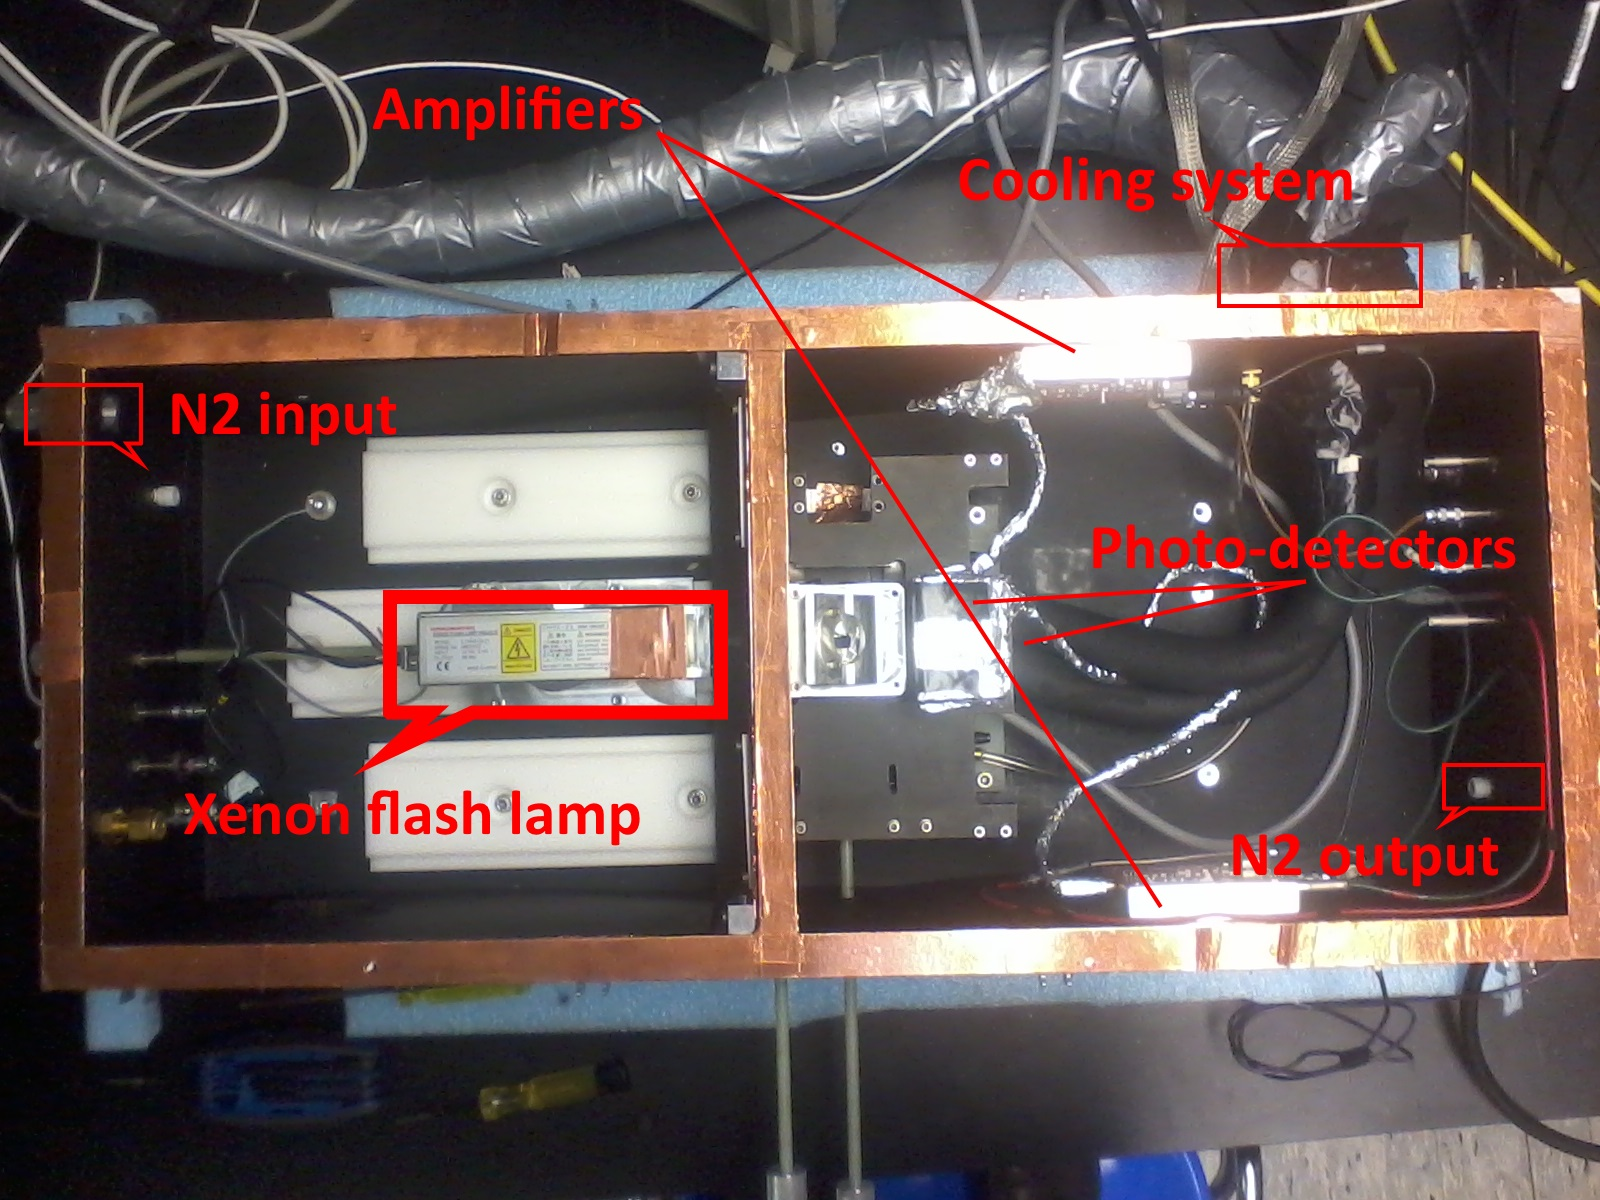
\includegraphics[totalheight=.35\textwidth,trim=0cm 7cm 0cm 2.5cm, clip=true,]{../Pictures/blabla/box.jpg}%trim=10cm 4cm 1cm 12cm, clip=true, 
  \caption{An aluminium box contains a \xfl and two photodetectors.}
  \label{fig:DN_AP_CT}
  \end{figure}
  
  The appendix A gives more details about the setup/The 
  
  \subsection{Treatment of the light}
  
  A Hamamatsu L11035-03-21 Xenon flash lamp module was utilized as a light source in a nitrogen-filled, light-tight box to simulate the 
  ultraviolet conditions of the future experiment. 
  The amount of light hitting the photodetectors was managed by a square wave pulse generator, otherwise saturation of the signal from the 
  photodetectors occurs. 
  \\
  To control light output, and thus the number of photons reaching the photodetectors, we could move out the lamp away from the surface of the detector 
  since intensity of light drops off as one over distance suqarred (make a plot). We could also set the voltage discharge on the lamp 
  by adding an external voltage supply line. 
  
  \begin{figure}[!hbtp]
  \centering
  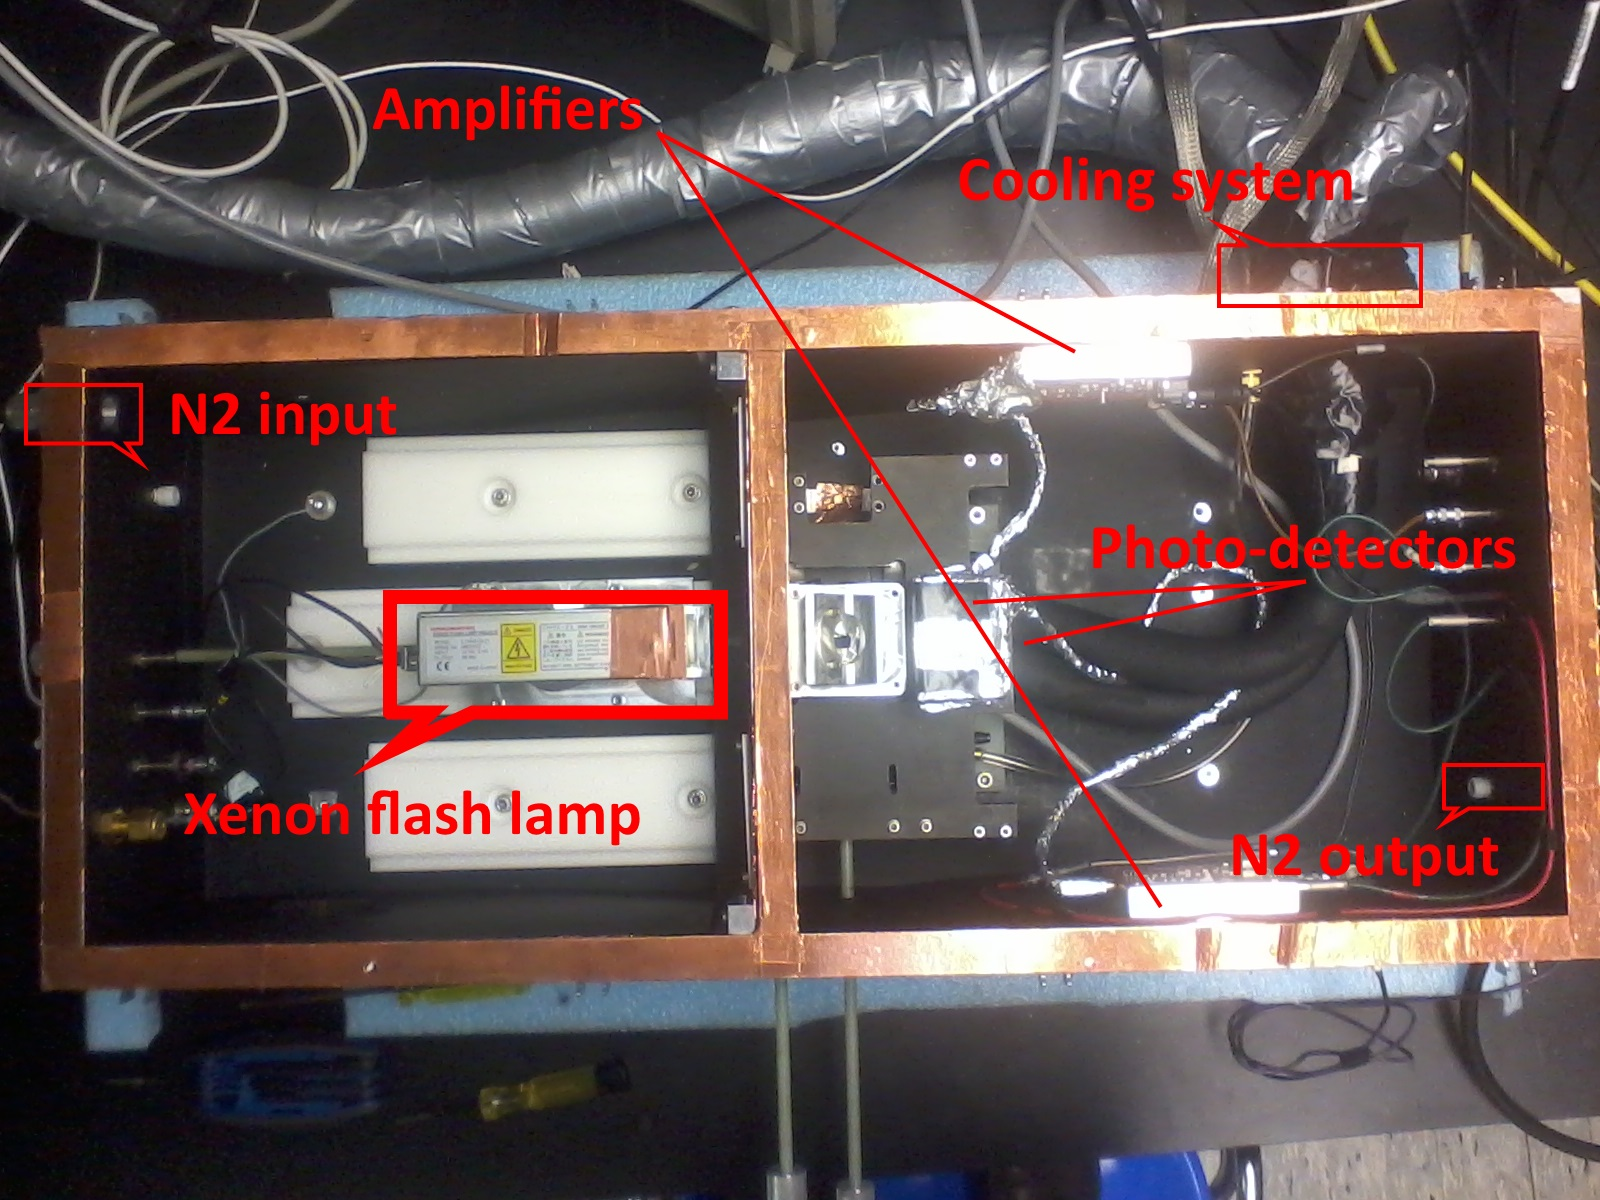
\includegraphics[totalheight=.35\textwidth,trim=0cm 7cm 0cm 2.5cm, clip=true,]{../Pictures/blabla/box.jpg}%trim=10cm 4cm 1cm 12cm, clip=true, 
  \caption{An external voltage supply line allow controling the \xfl.}
  \label{fig:external_supply_line}

  For all our measurements, the position of the lamp and the external voltage were set at 20 mm from the metal divider of the box and at 2.8 V, respectively.
  Then the light was collimated by a 5 mm hole, filtered, and then interacts with a beam splitter (BS). The beam splitter separated the 
  incoming beam into two 
  equal beams which reached the surface of each photodetector at the same time. 
  \\
  Two pictures side by side. one bs and other filter.  
  
  \begin{figure}[!hbtp]
  \centering
  \begin{subfigure}{.5\textwidth}
    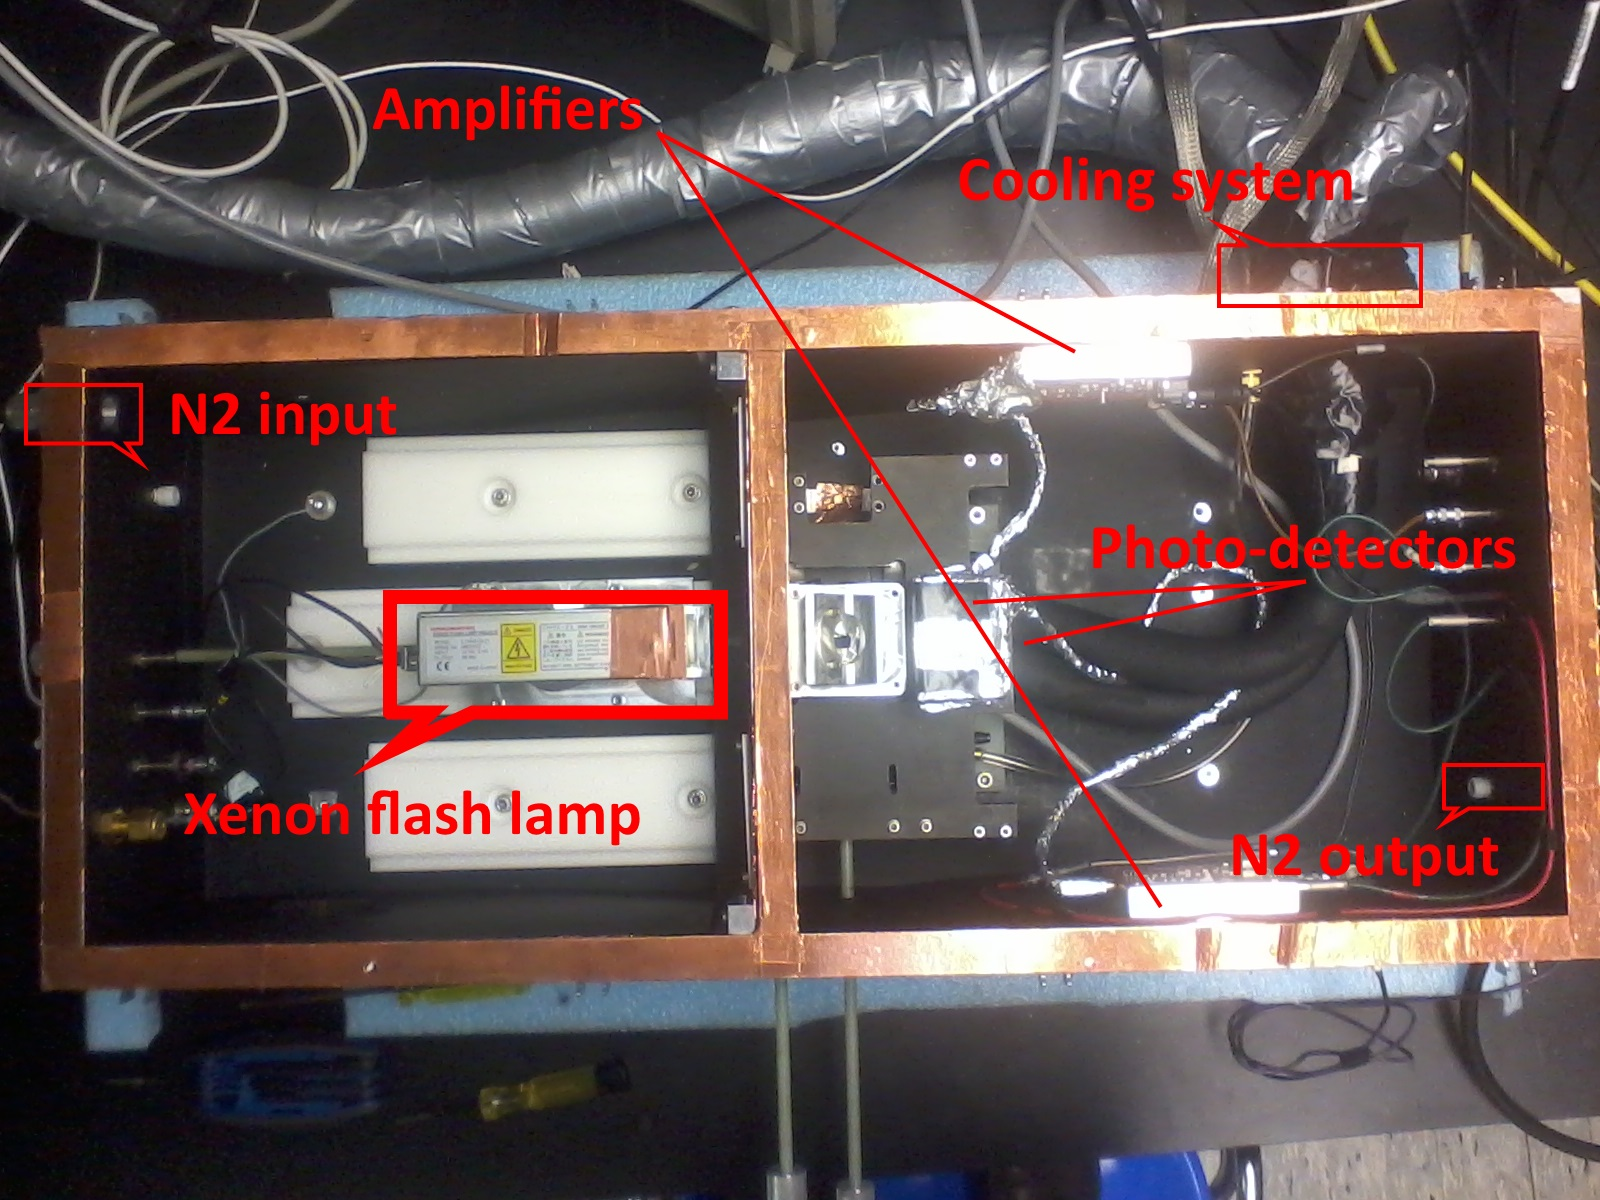
\includegraphics[totalheight=.35\textwidth,trim=0cm 7cm 0cm 2.5cm, clip=true,]{../Pictures/blabla/box.jpg}%trim=10cm 4cm 1cm 12cm, clip=true, 
    \caption{The incoming beam reachs the surface of each detectors due to the beam splitter.}
    \label{fig:beam_splitter}
  \end{subfigure}%
  \begin{subfigure}{.5\textwidth}
    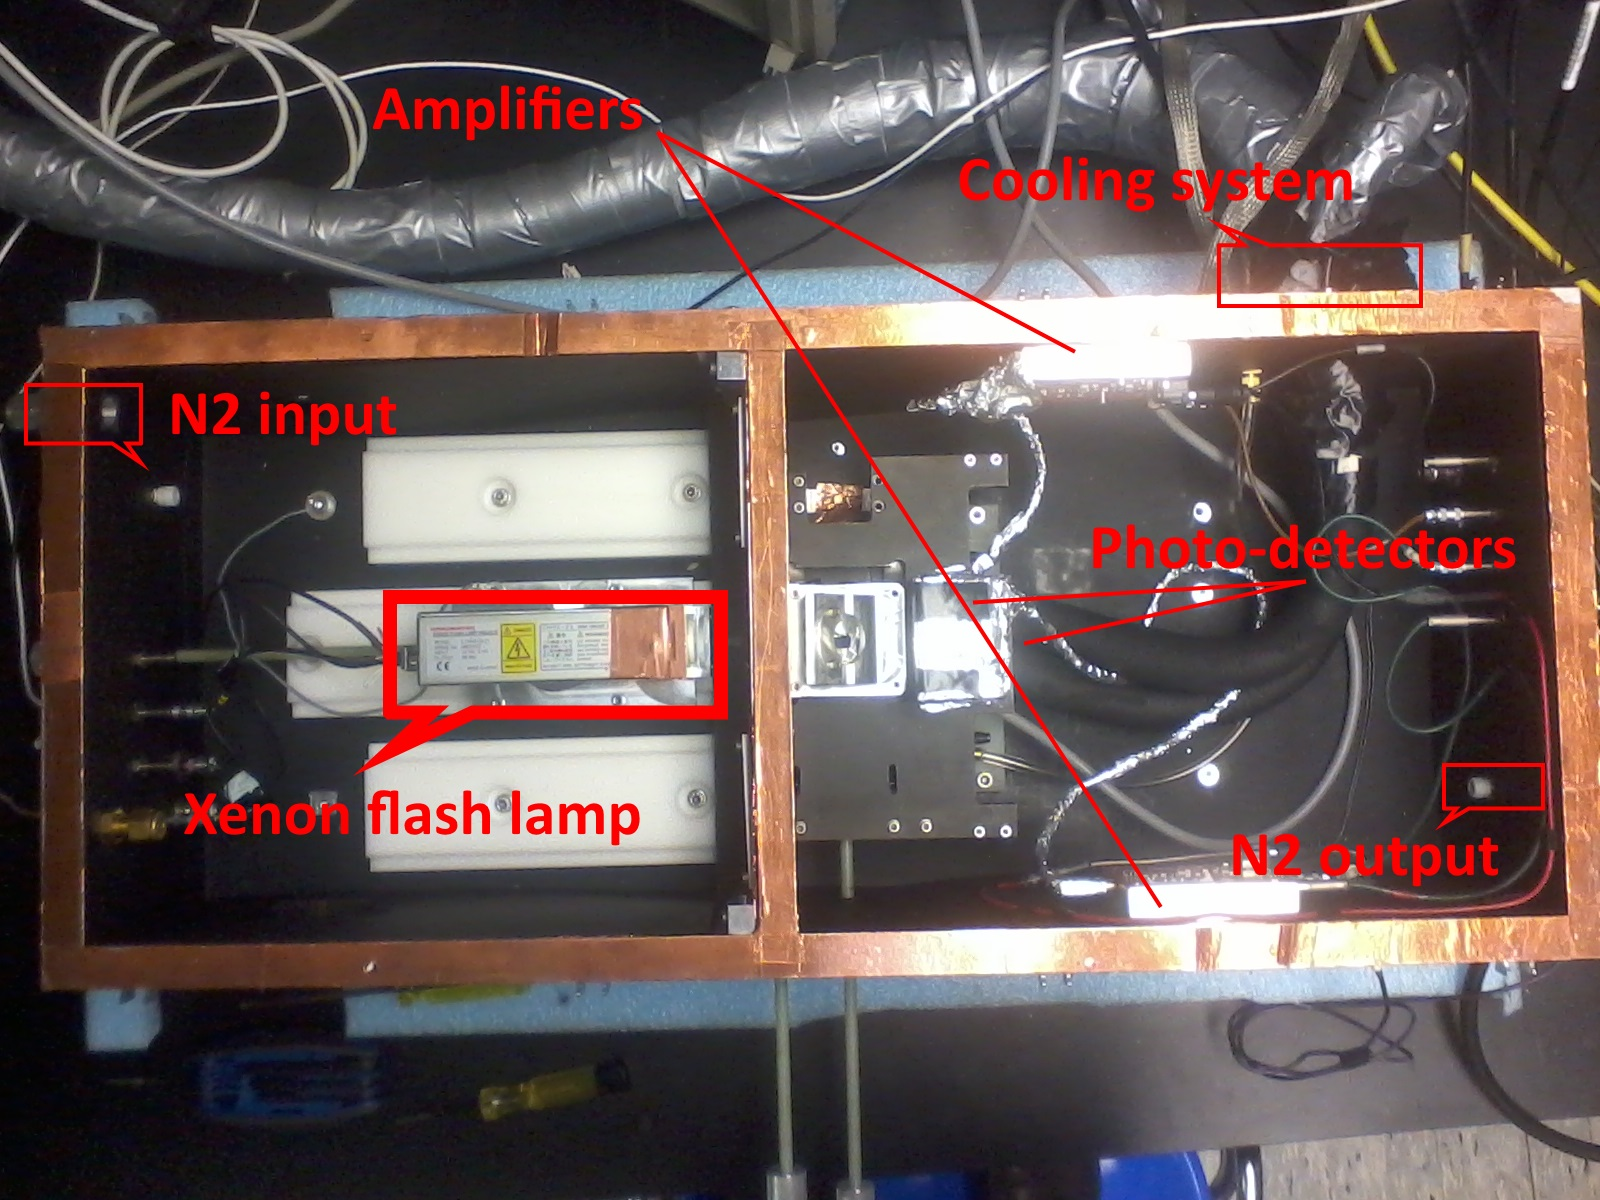
\includegraphics[totalheight=.35\textwidth,trim=0cm 7cm 0cm 2.5cm, clip=true,]{../Pictures/blabla/box.jpg}
    \caption{One of the three filters used to atenuate the light.}
    \label{fig:filters}
  \end{subfigure}
  \end{figure}
  
  
  The \xfl emits a spectrum of light in visible-light visible regions. With an external power supply, the lamp send a flash of 10 µs each 
  10 ms. The appendix gives the pulse shape of the \xfl.\\
  A filter select the 175 nm wavelength (UV region). 
  A test was made to ensure that no visible light from that lamp could reach the photo-detectors\footnote{name.} sensitive to the visible wavelength. 
  Otherwise such light could have got wronf our results for the efficiency.
  This filter also attenuated the light of the \xfl by 20\%. Then two other 
  identical filters were added to provide additional attenuations (the light reaching the photo-detectors was still too intense). 
  \\
  
  \centering
  \begin{figure}[!hbtp]  
    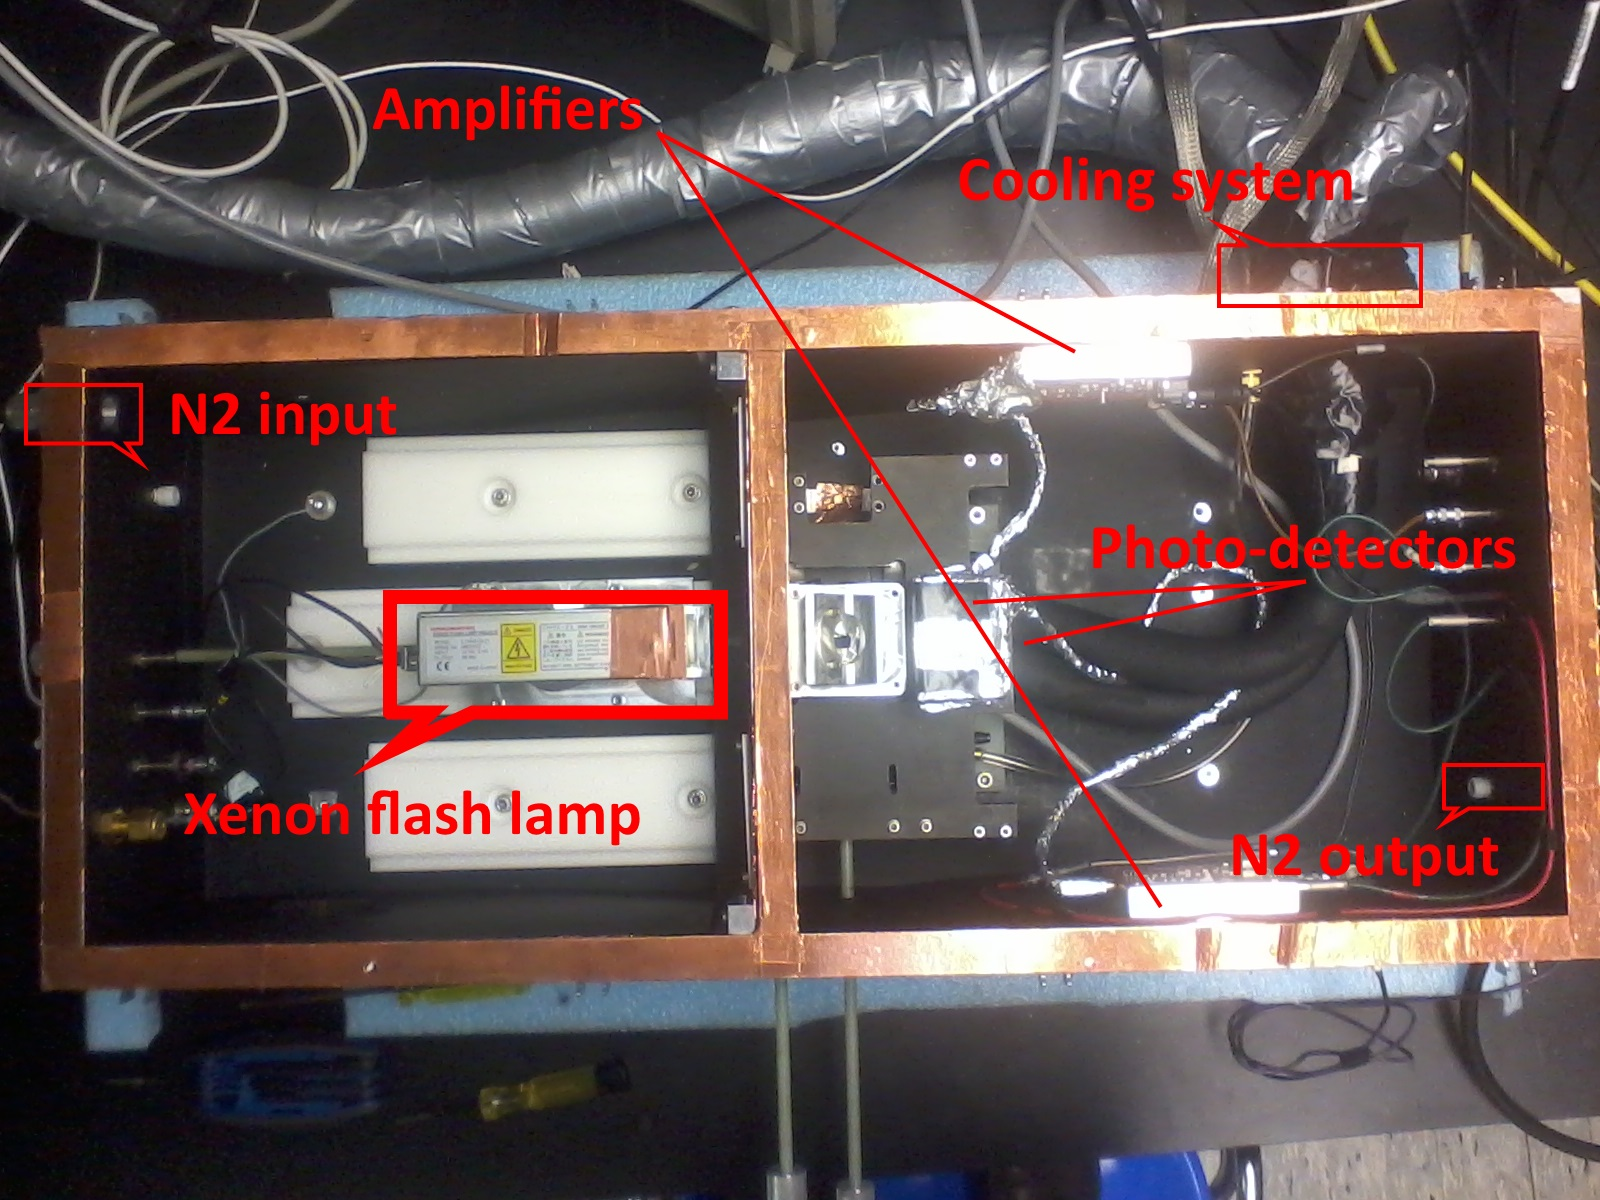
\includegraphics[totalheight=.35\textwidth,trim=0cm 7cm 0cm 2.5cm, clip=true,]{../Pictures/blabla/box.jpg}
    \caption{The closest filter near the lamp select the VUV region.}
    \label{fig:filter_specification}
  \end{figure}
  
  As photons of this wavelength have an attenuation length of only a few mm, the box was filled with N2 gas. The second advanatge of using 
  N2 is to avoid frost on the surface of the cooling photo-detectors on the bottom.
   
  \centering
  \begin{figure}[!hbtp]  
    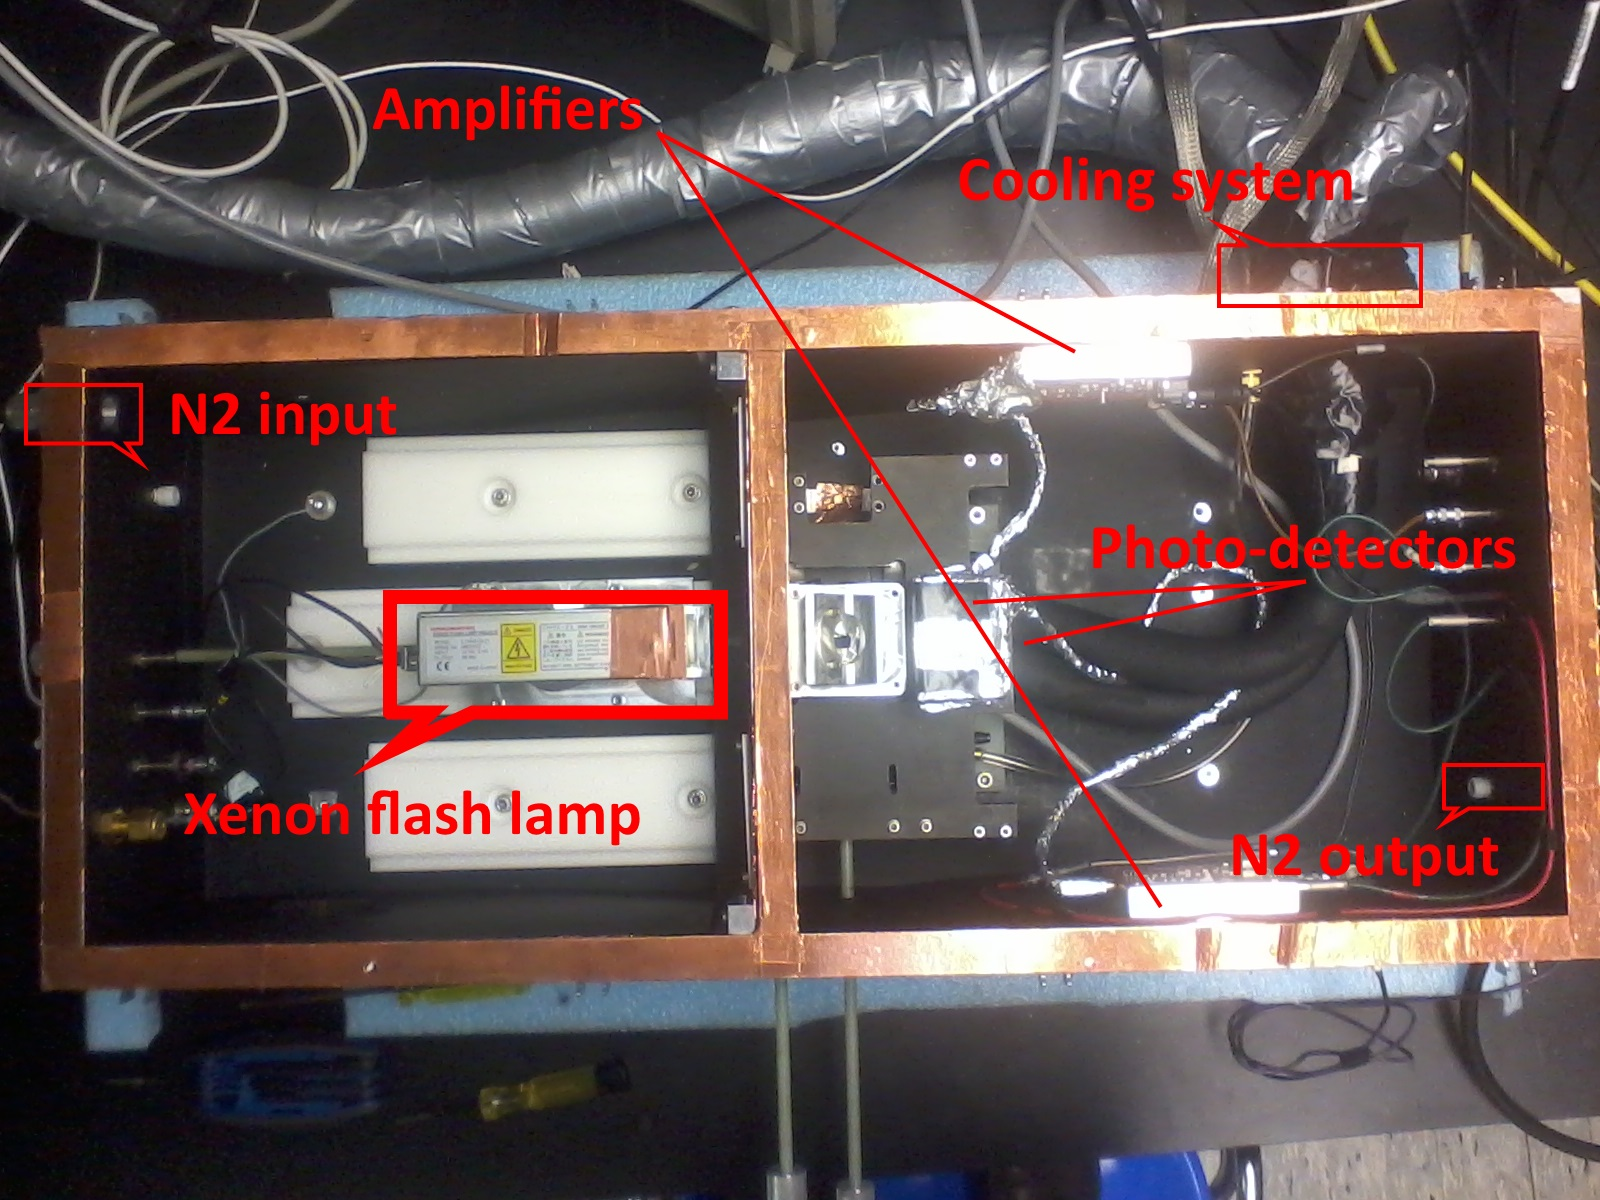
\includegraphics[totalheight=.35\textwidth,trim=0cm 7cm 0cm 2.5cm, clip=true,]{../Pictures/blabla/box.jpg}
    \caption{N2 from that bottle fills the box.}
    \label{fig:filter_specification}
  \end{figure}
  
  
  \subsection{Photo-detectors and cooling system}
  
  Two photo-detectors were used for each run to calculate the efficiency.\\
  The one on the top allow ensuring that the light remind constant over the time. For that we used a VUV2 SIPM from Hammatsu.
  
  \centering
  \begin{figure}[!hbtp]  
    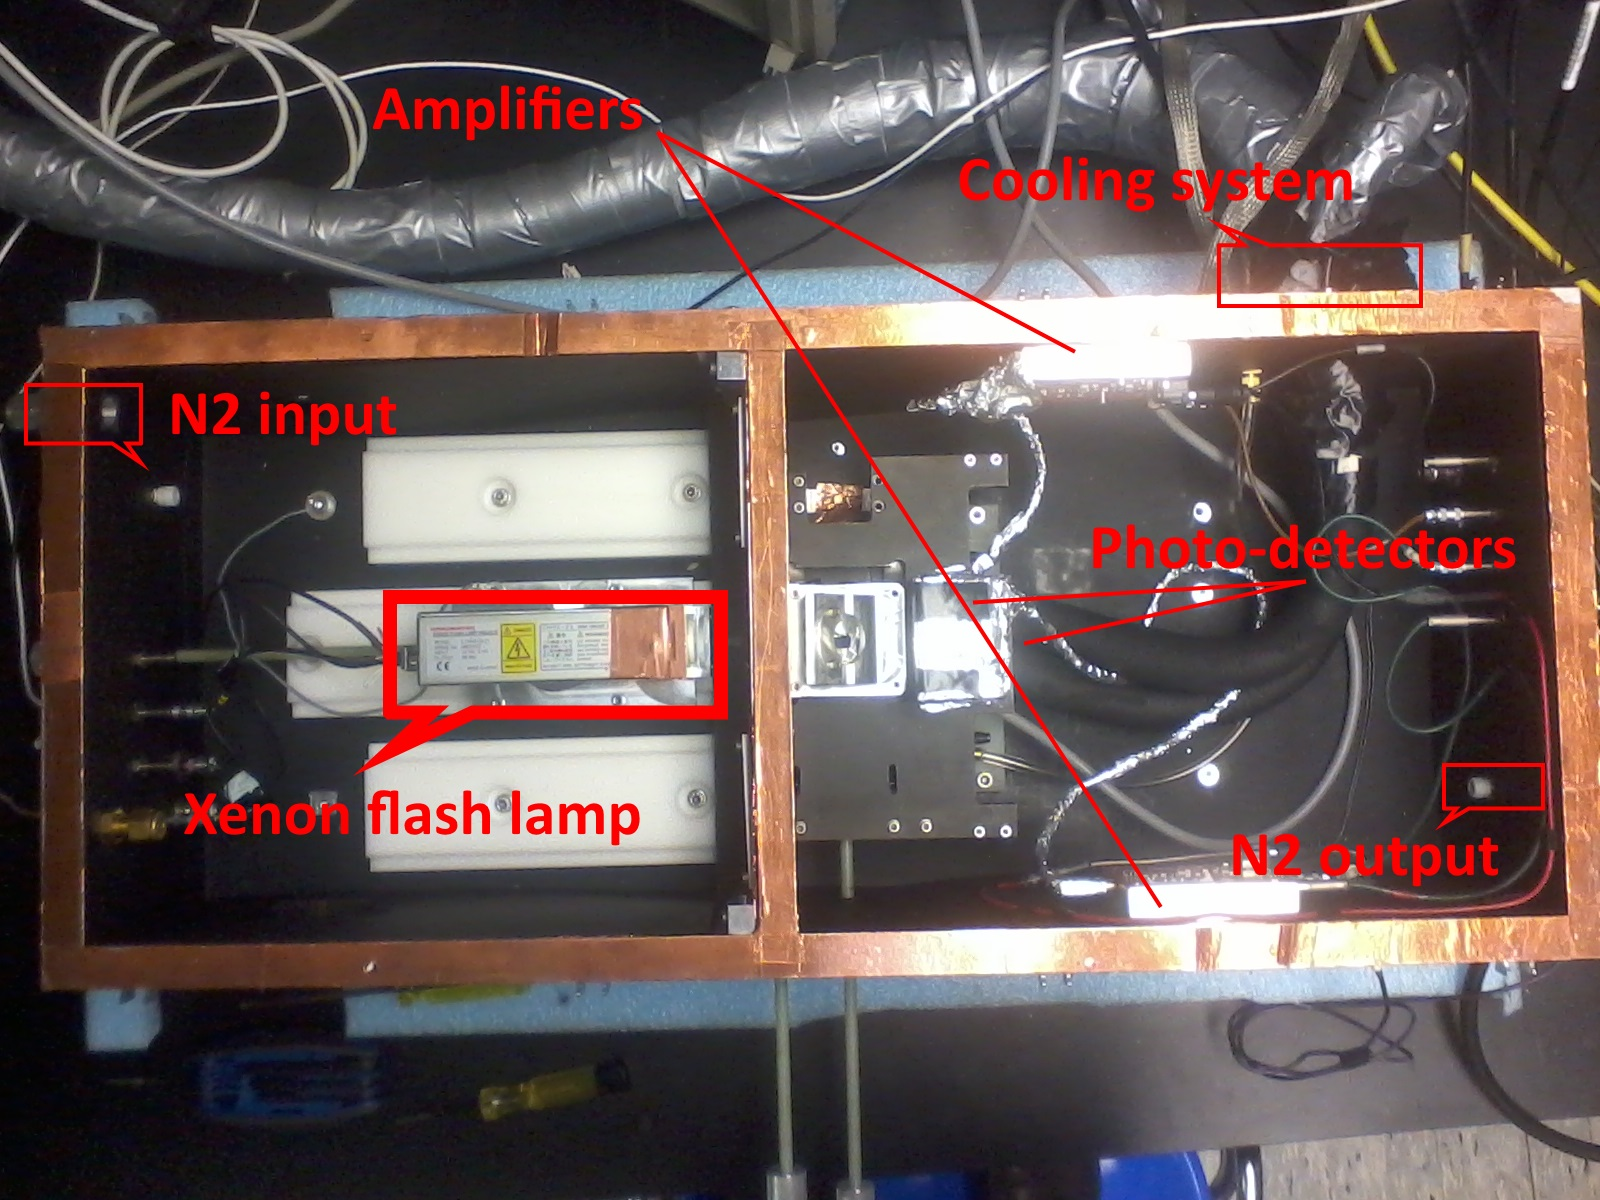
\includegraphics[totalheight=.35\textwidth,trim=0cm 7cm 0cm 2.5cm, clip=true,]{../Pictures/blabla/box.jpg}
    \caption{A VUV2 SiPM on the top let check if the  light from the lamp is constant.}
    \label{fig:top}
  \end{figure}
  
  We choose that one beacaue the dark noise rate\footnote{see section.} is quiet low at room temperature (20C). So it is possible 
  to calculate the relative efficiency of that detector at such temperature./So the efficiency of that photo-detector is not perturbé
  due to a high rate of dark noise\footnote{see section.}
  
  The photo-detector on the bottom were characterize (calculation of the efficiency at -100C, of the dark noise and the number of 
  correlated pulse rate).\\
  A cooling system allow working at such low temperature and the photo-detector to characterize was laying on a chock. A plastic board 
  with bad termo conductivity holds the whole cooling shock to avoid thermal flee.\\
    
  \begin{figure}[!hbtp]
  \centering
  \begin{subfigure}{.5\textwidth}
    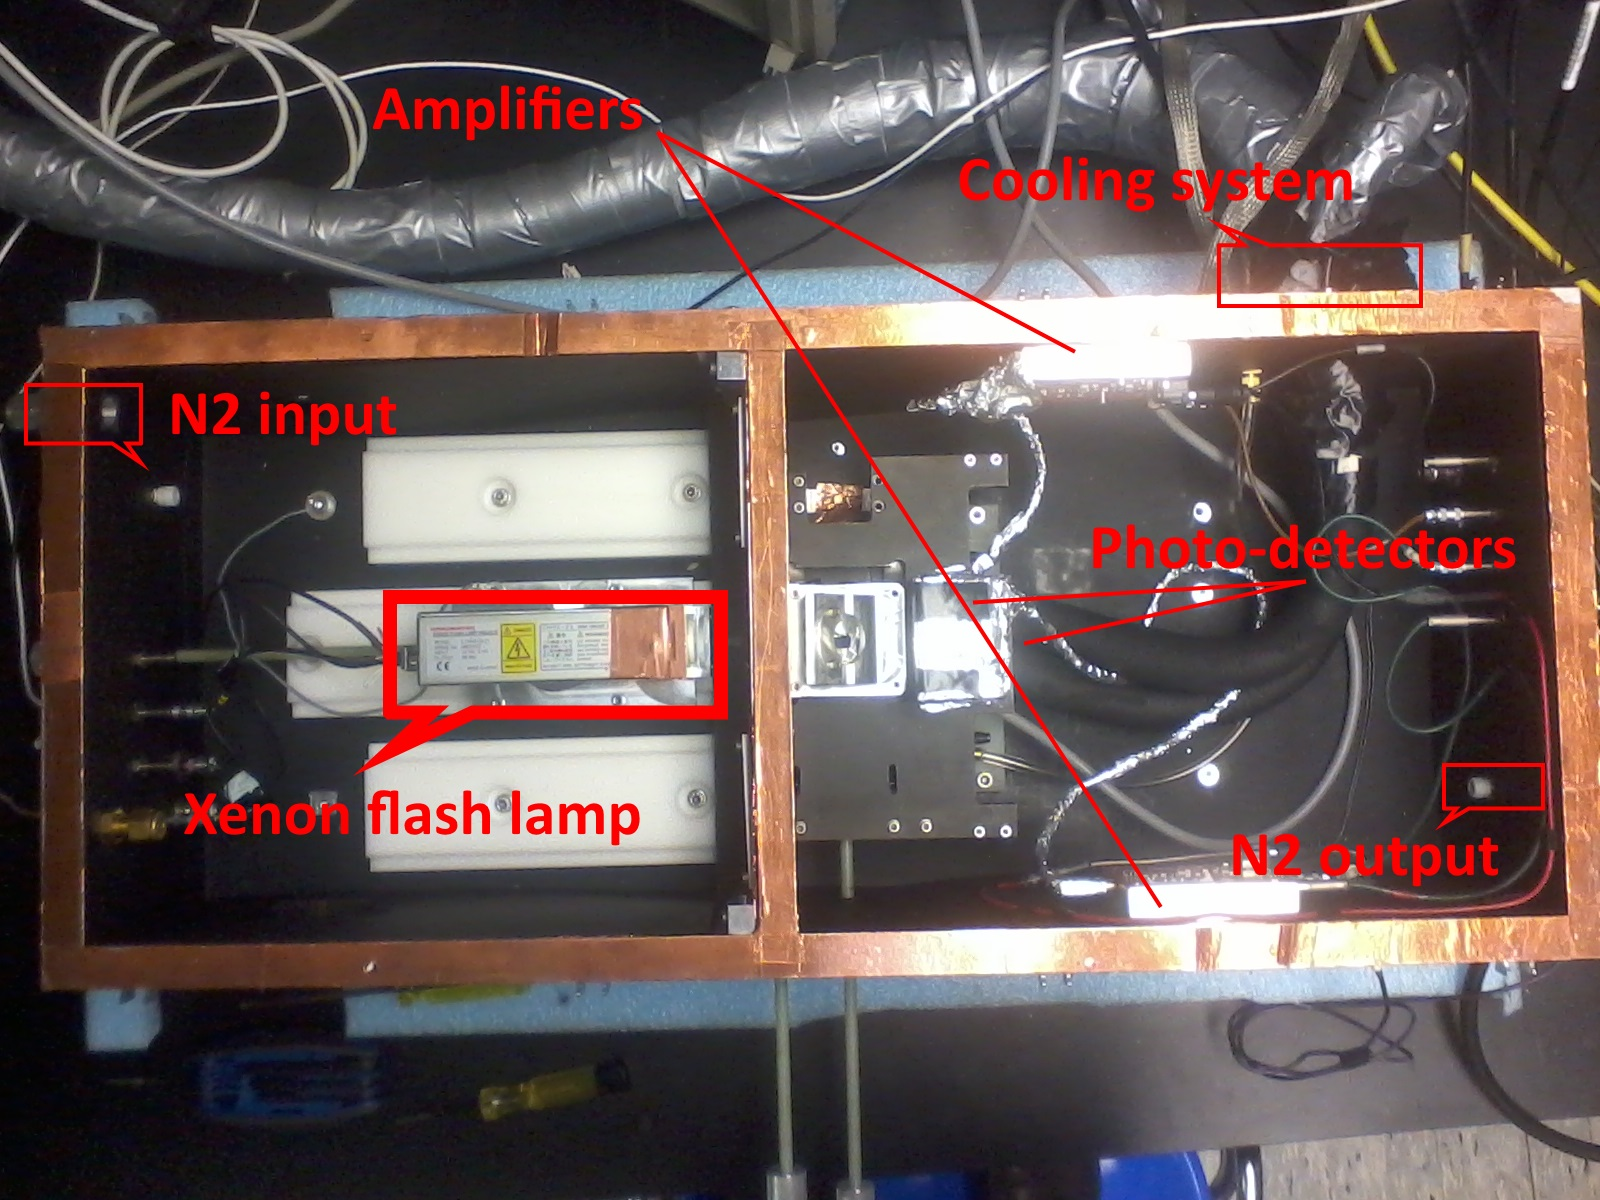
\includegraphics[totalheight=.35\textwidth,trim=0cm 7cm 0cm 2.5cm, clip=true,]{../Pictures/blabla/box.jpg}%trim=10cm 4cm 1cm 12cm, clip=true, 
    \caption{The cooling system let work up to -110C.}
    \label{fig:beam_splitter}
  \end{subfigure}%
  \begin{subfigure}{.5\textwidth}
    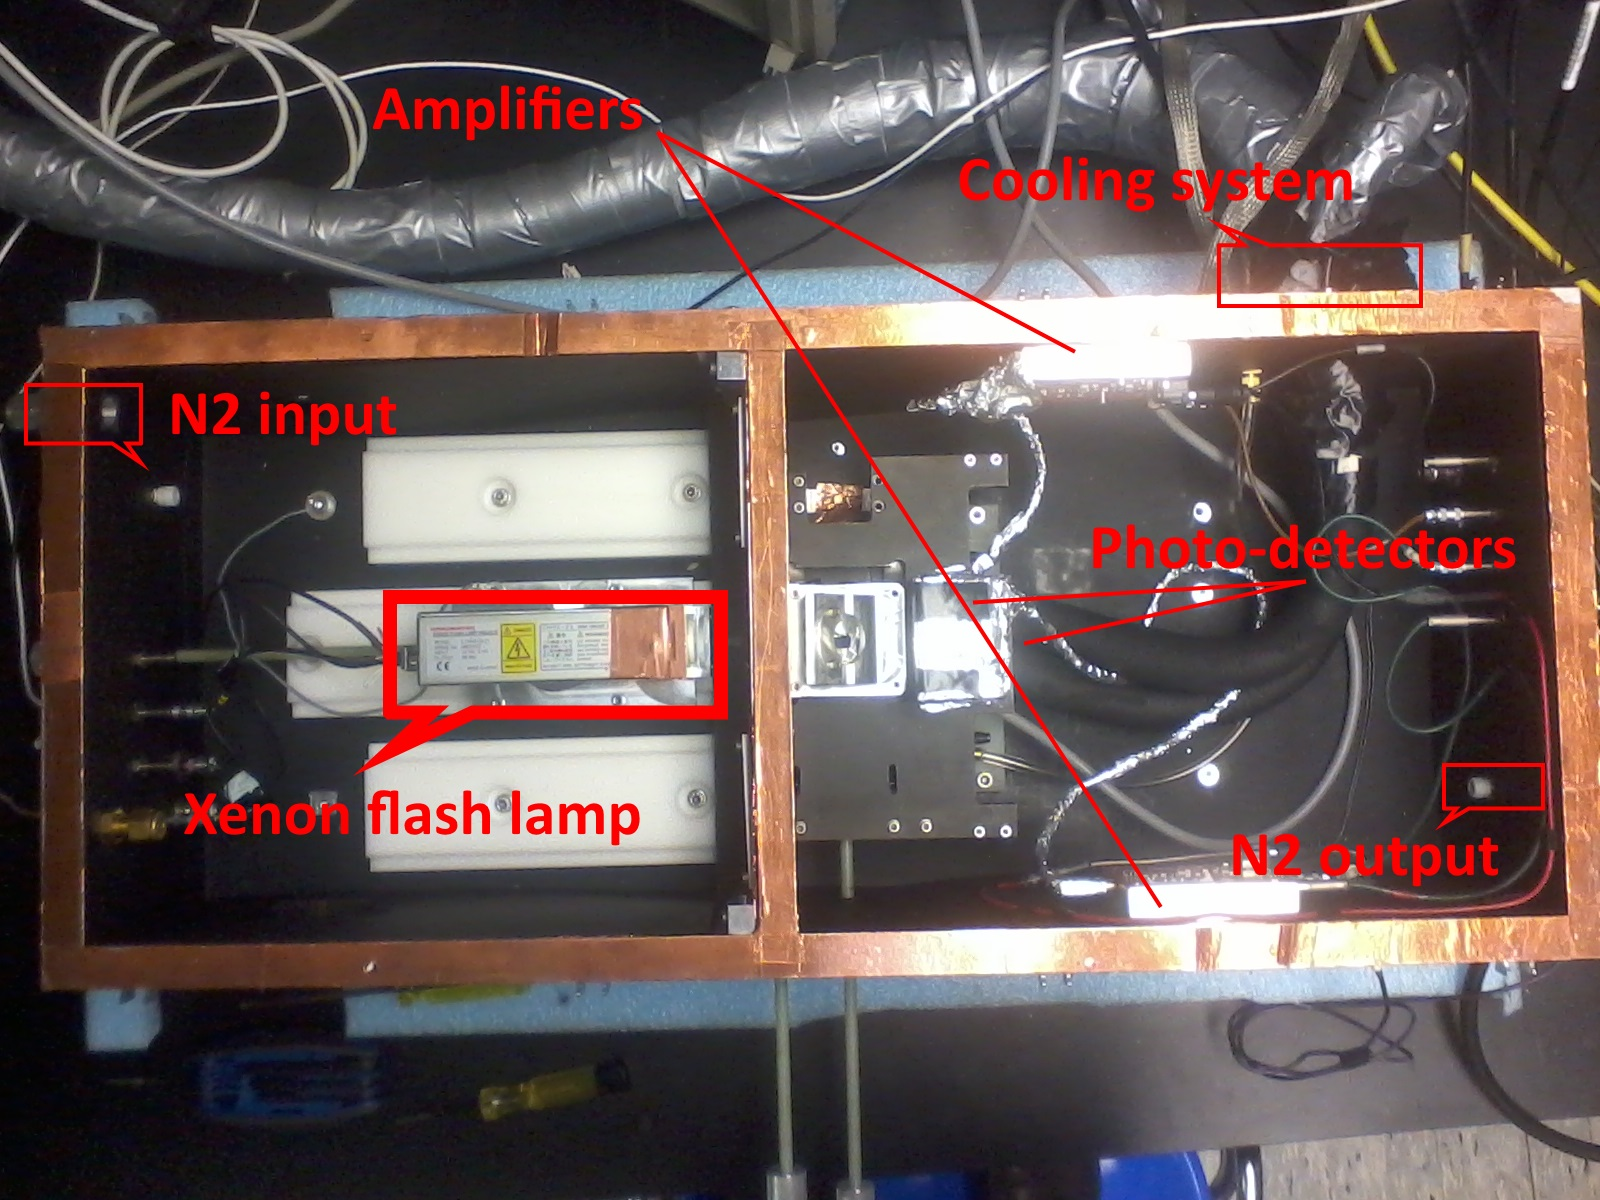
\includegraphics[totalheight=.35\textwidth,trim=0cm 7cm 0cm 2.5cm, clip=true,]{../Pictures/blabla/box.jpg}
    \caption{ VUV3 SIPM of HAMMAMATSU.}
    \label{fig:cooing system}
  \end{subfigure}
  \end{figure}  
  
  Several different SiPM were tested to select the best one/ the more suitable one for nEXO.
  
  \begin{figure}[!hbtp]
  \centering
  \begin{tabular}{|l|c|c|c|}
  \hline
  D\'etecteur SiPM (diff\'erents fournisseurs) &Efficacit\'e &Dark Noise &Cross Talk + After Pulse\\
  \hline
  MPPC VUV2/MEG &oui &oui &oui\\
  \hline
  MPPC VUV3/MEG &non &non &non\\
  \hline
  MPPC cooted &non &- &-\\
  \hline
  KETEK 1 &- &non &non\\
  \hline
  KETEK 2 & &non &non\\
  \hline
  FDK VUV &non &non &non\\
  \hline
  FBK &- &non &non\\
  \hline
  \end{tabular}
  \end{figure}
  
  \subsection{Temperature sensors and automatisation}
  
  We noticed that the whole bow were cooling down over time when we were working at -100C, even the plastic holder.\\
  To check if that physical phenomena could have an impact on our reseults for the efficiency 10 tempererature sensors were installed inside 
  the box after calibrating them\footnote{See appendix for more details.}\\
  At was possible to record all the temperatures by using such device. 
  
  \begin{figure}[!hbtp]
  \centering
  \begin{subfigure}{.5\textwidth}
    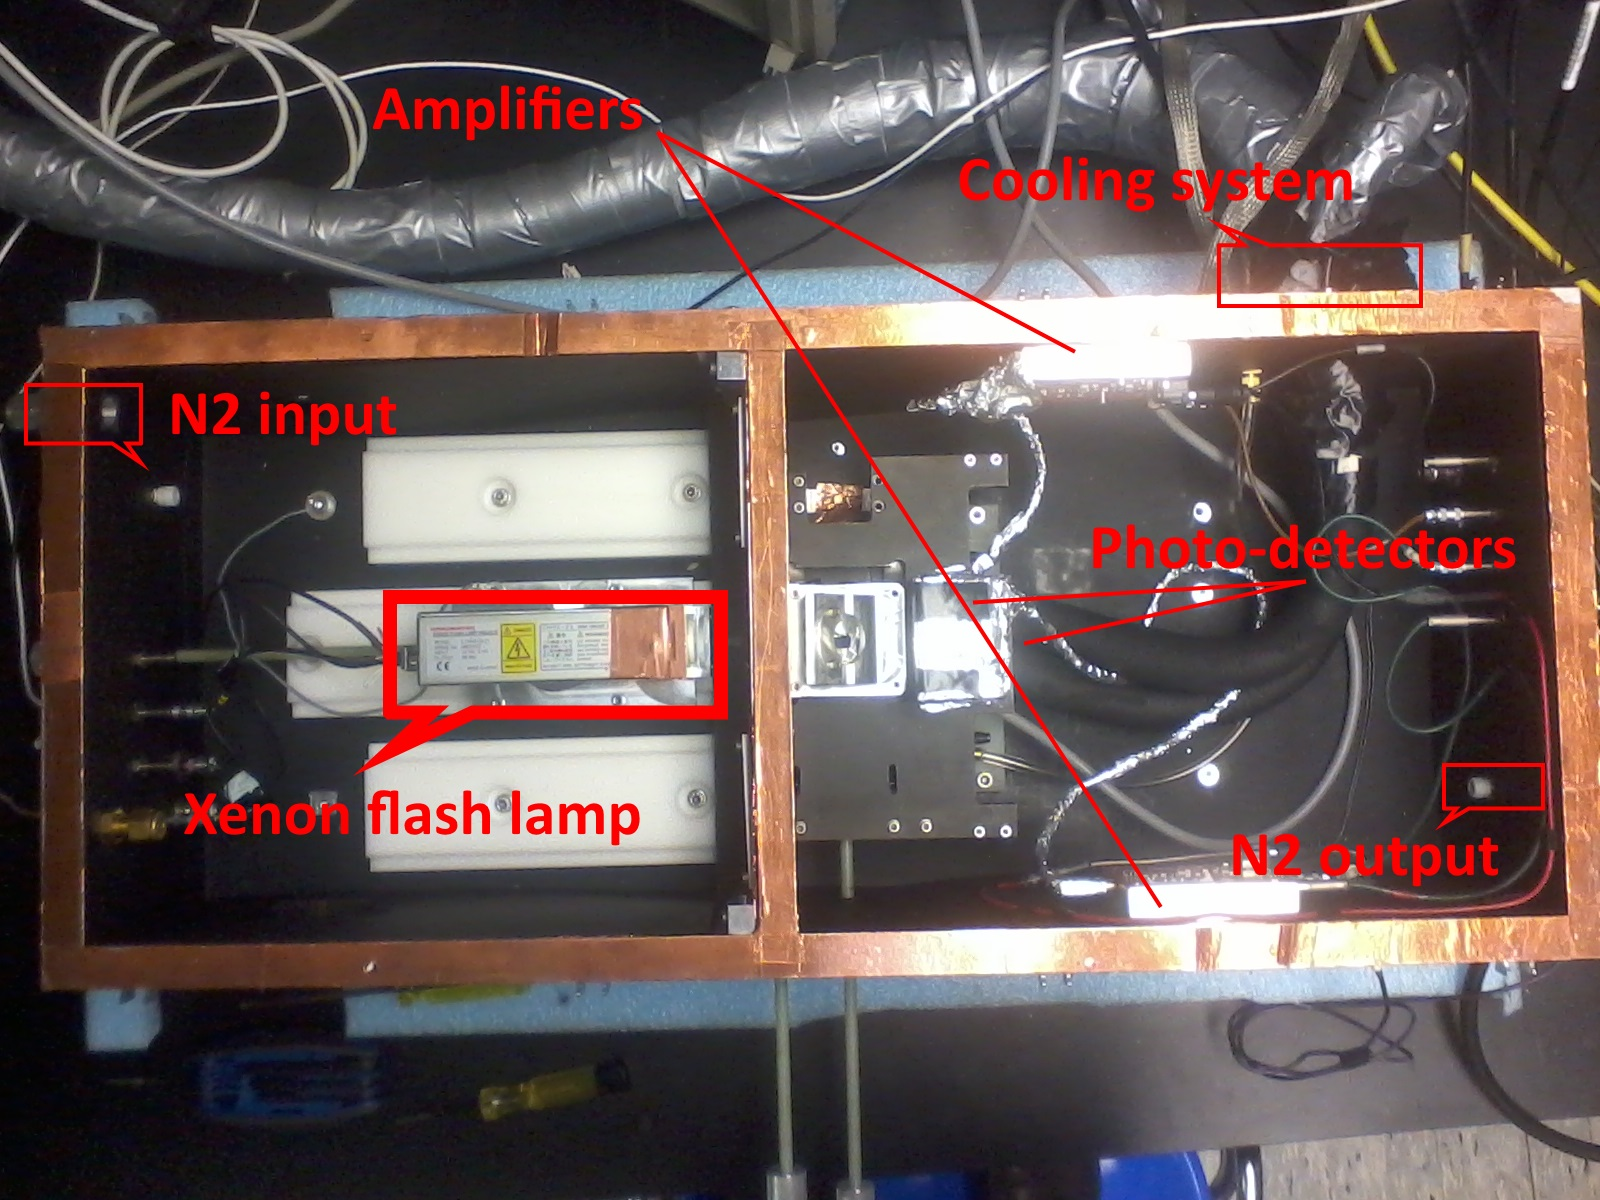
\includegraphics[totalheight=.35\textwidth,trim=0cm 7cm 0cm 2.5cm, clip=true,]{../Pictures/blabla/box.jpg}%trim=10cm 4cm 1cm 12cm, clip=true, 
    \caption{On of the ten tempearture sensors.}
    \label{fig:beam_splitter}
  \end{subfigure}%
  \begin{subfigure}{.5\textwidth}
    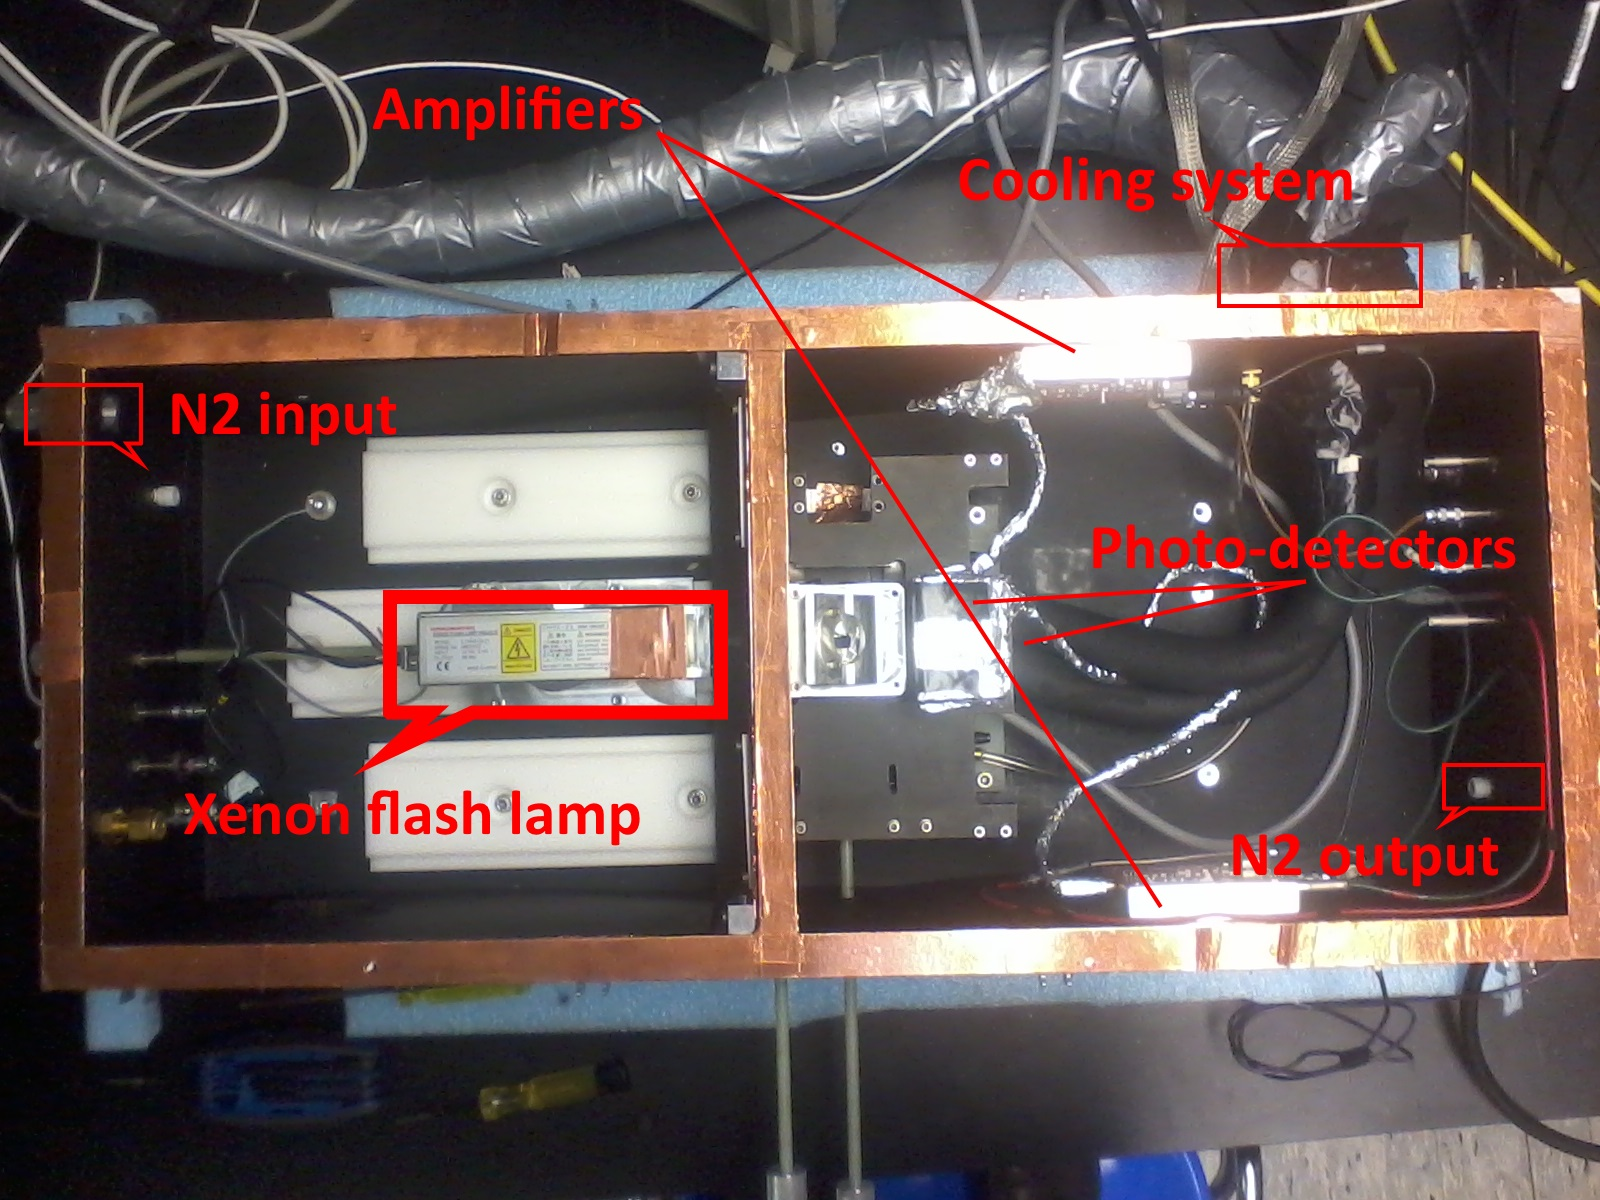
\includegraphics[totalheight=.35\textwidth,trim=0cm 7cm 0cm 2.5cm, clip=true,]{../Pictures/blabla/box.jpg}
    \caption{That device let record the different temperature.}
    \label{fig:filters}
  \end{subfigure}
  \end{figure}
  
  Also a program were written to set the volatge sended to the photo-detectors, to record the current from them and to record the 
  temperature at differentparts of the box. 
  
  \section{Silicon Photo-Multiplier}
  
  A Silicon photomultiplier (SiPM) is a photon detector (detect light). Many groups concerning sudy their applicability in many different 
  fields such as high-energy, physics calorimetry, astrophysics or medical imaging \ref{}.\\
  Compared to EXO experiment which uses conventional vacuum tube PM (PhotoMultiplier), SiPMs for nEXO experiment are a very promising 
  alternative because of the very good properties of such devices:
  
  \begin{itemize}
   \item SiPMs are insentive to magnetic fields,
   \item SiPMs' operation voltage is far lower than PMs,
   \item SiPMs' gain is \(10^6 - 10^7\) higher than PMs' gain\footnote{The resolution of energy and so the gain of the SiPM is a 
   reason why nEXO choose them},
   \item SiPMs have a very good time (ns) and photon-counting resolutions (µm) due to the size of the one pixel.
  \end{itemize}

  %SiPM properties like high gain \(10^6 - 10^7\) and sensitivity, and very good time (ns) and photon-counting (nm) resolutions
  %\.
  
  \subsection{Structure}
  
  This device consists a matrix of typically 1000 independent and equal mirco-cells (pixels) per mm\texttwosuperior{}. A pixel consists the basic 
  element of SiPMs.\\
  Each pixel are connected in parallel. They are formed out of an Avalanche PhotoDiode (APD) and a quenching resistor which is 
  connected in series to an APD. 
  
  \begin{figure}[!hbtp]
  \centering
  \begin{subfigure}{.5\textwidth}
    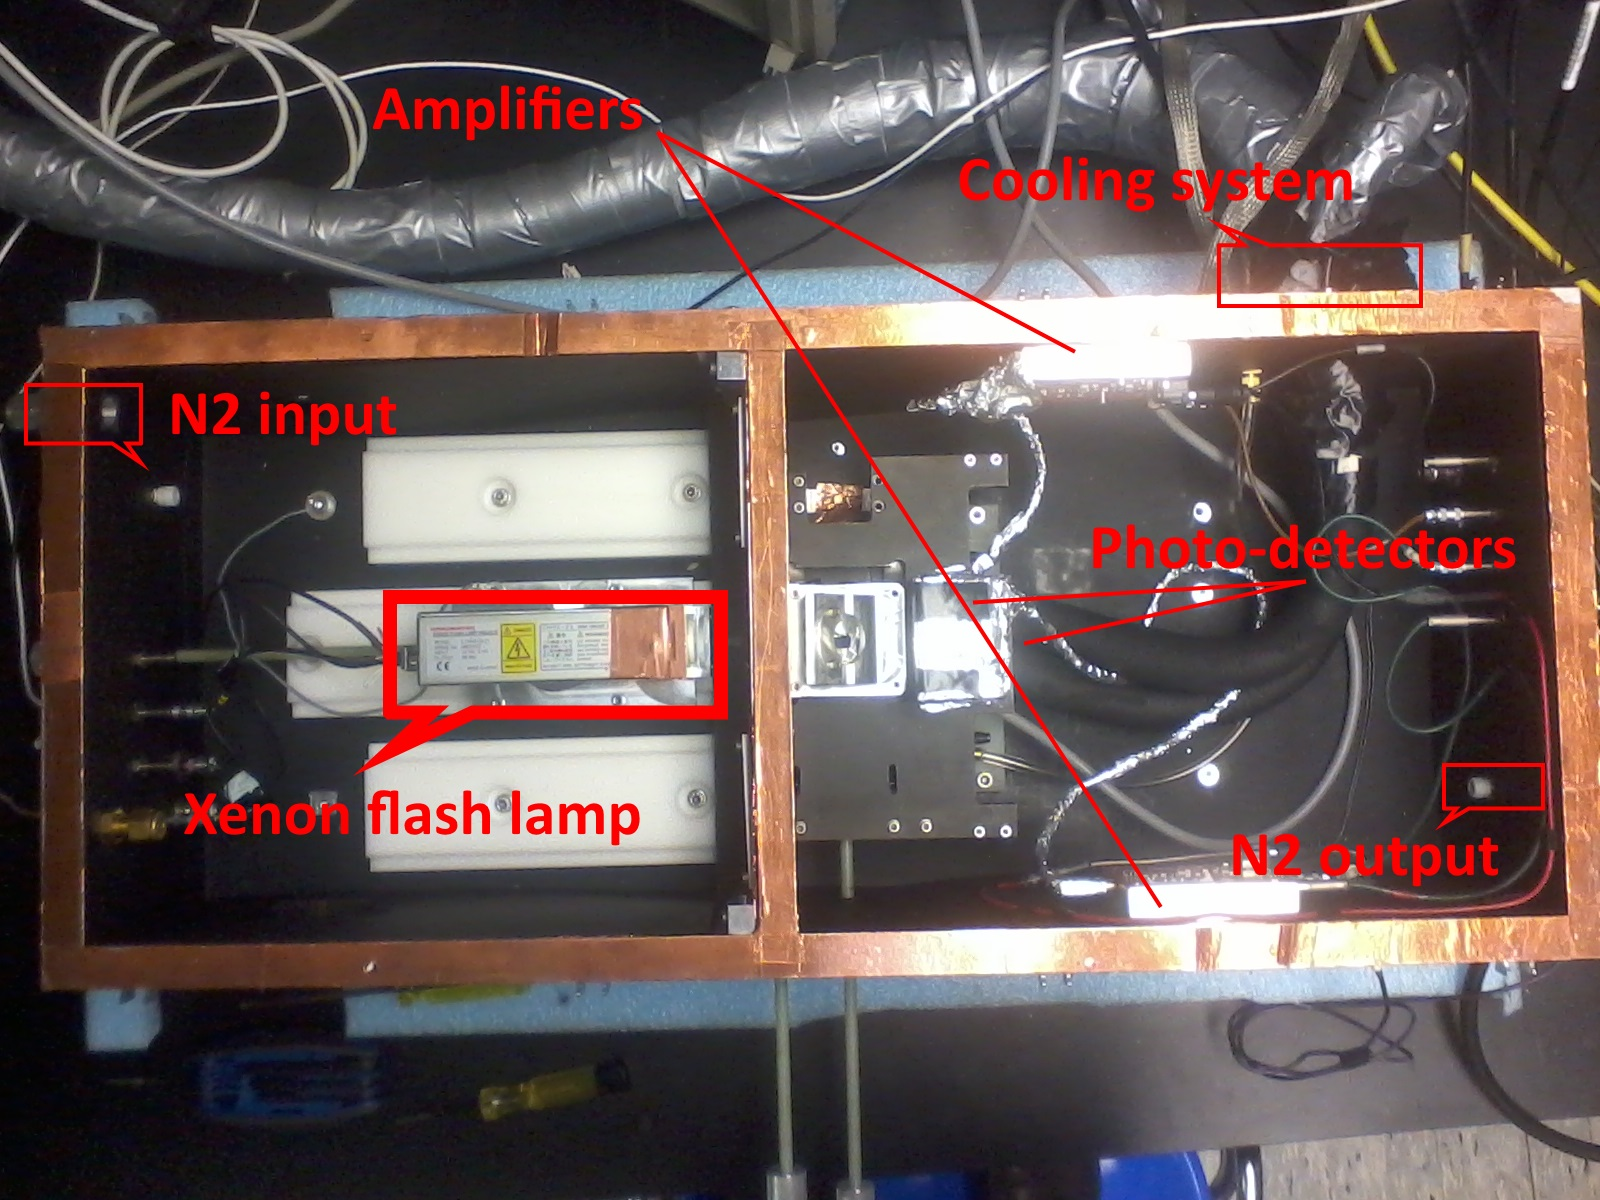
\includegraphics[totalheight=.35\textwidth,trim=0cm 7cm 0cm 2.5cm, clip=true,]{../Pictures/blabla/box.jpg}%trim=10cm 4cm 1cm 12cm, clip=true, 
    \caption{A SiPM from HAMMAMATSU VUV sensitive.}
    \label{fig:SiPM}
  \end{subfigure}%
  \begin{subfigure}{.5\textwidth}
    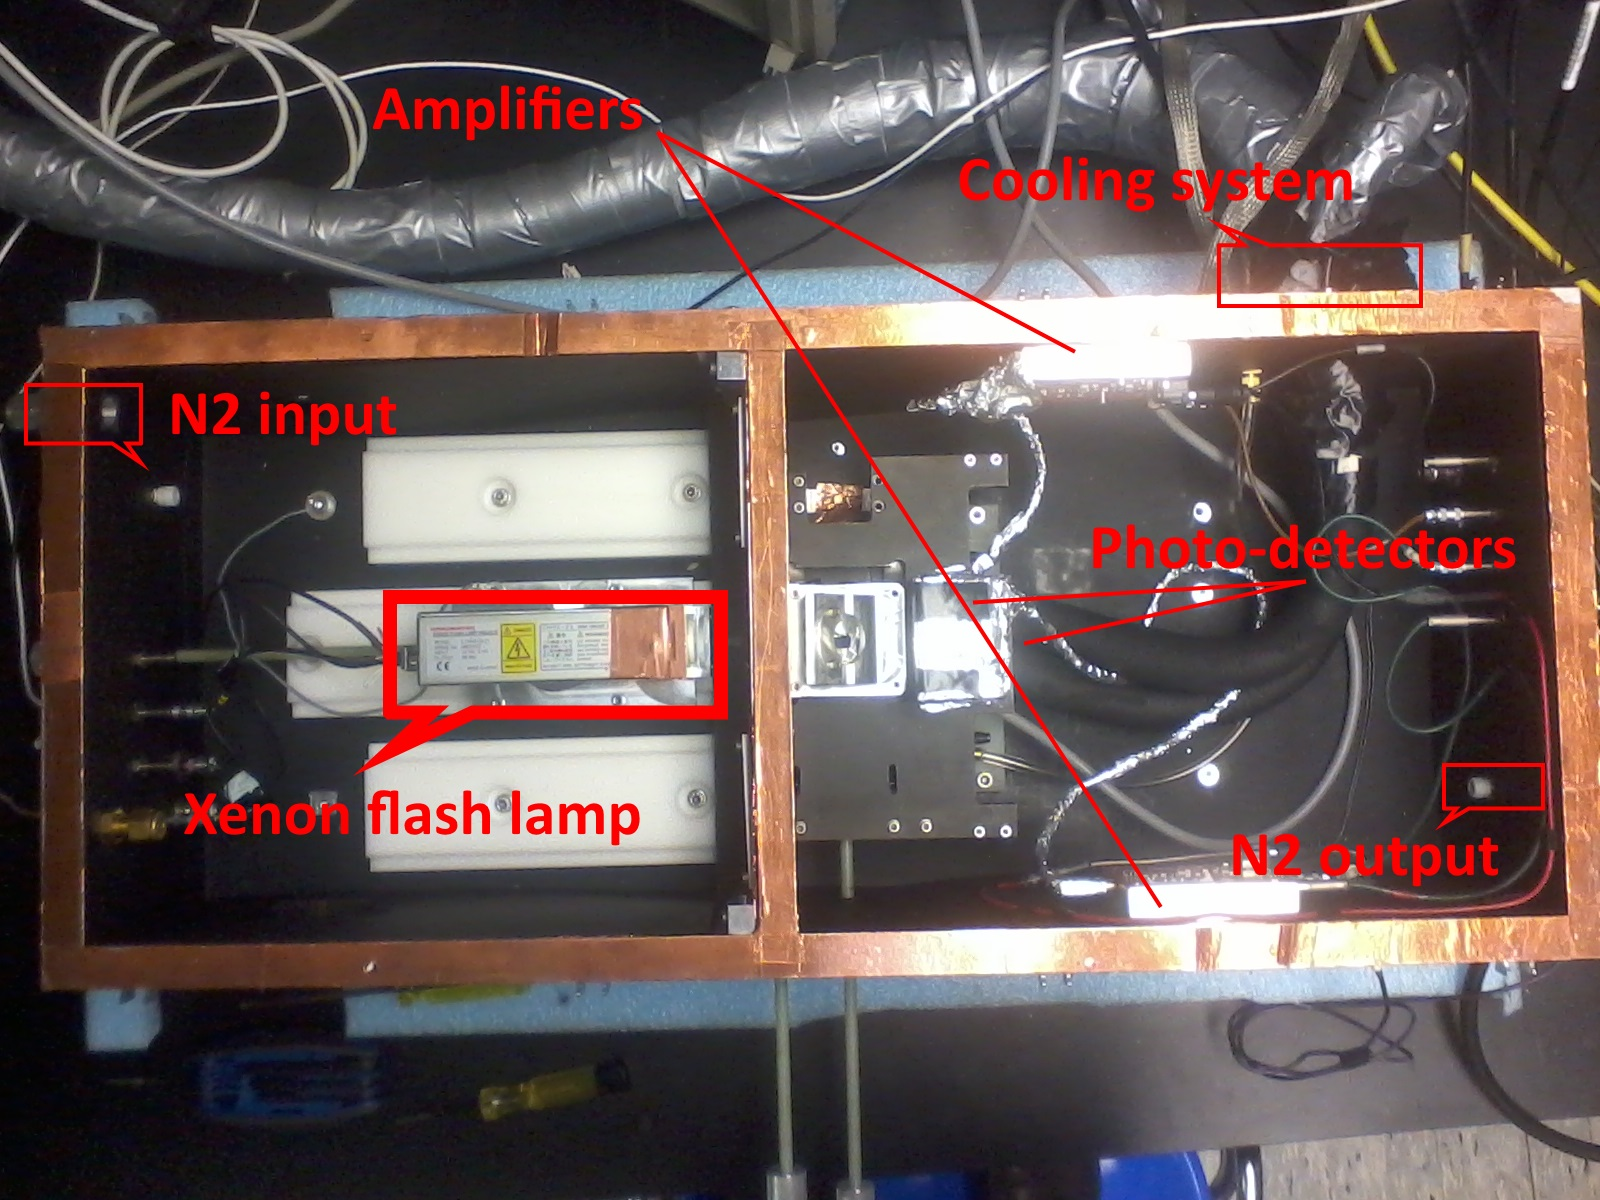
\includegraphics[totalheight=.35\textwidth,trim=0cm 7cm 0cm 2.5cm, clip=true,]{../Pictures/blabla/box.jpg}
    \caption{Equivalent circuit.}
    \label{fig:electrical_circuit}
  \end{subfigure}
  \end{figure}

  %global electrical circuit with amplifier and scope? 
  \subsection{Basic operation}\label{basic operation}
  
  Each pixel in a SiPM outputs a pulse at the same amplitude when it detects a photon. 
  A pulse produced from one pixel do not vary with the number of incident photons firing that pixel. 
  All pixels are connected to the same output channel. The total output signal is equal to the sum of those from the indidividual pixels 
  firing by photons.
  \\
  
  For example,if four photons are incident on different pixels and detected at the same time, then the SiPM outputs a signal whose ampli-
  tude equals the height of the four superimposed pulses.

  %So the number of output pulses is always one regardless the number of incoming photon. This means that MPPC output linearity gets worse 
  %as more photons are incident on the MPPC such as when two or more photons enter one pixel. This makes it essential to select an MPPC 
  %having enough pixels to match the number of incident photons.
 
  One feature of the SiPM is that each APDs operate in Geiger mode.
  
  \subsection{Physical APD's operation.}
  
  \subsubsection{PN Junction}
  A pixel is a photodiode and a photodiode has the structure of a PN junction \ref{biblio} :
  
  \begin{figure}[!hbtp]
  \centering
  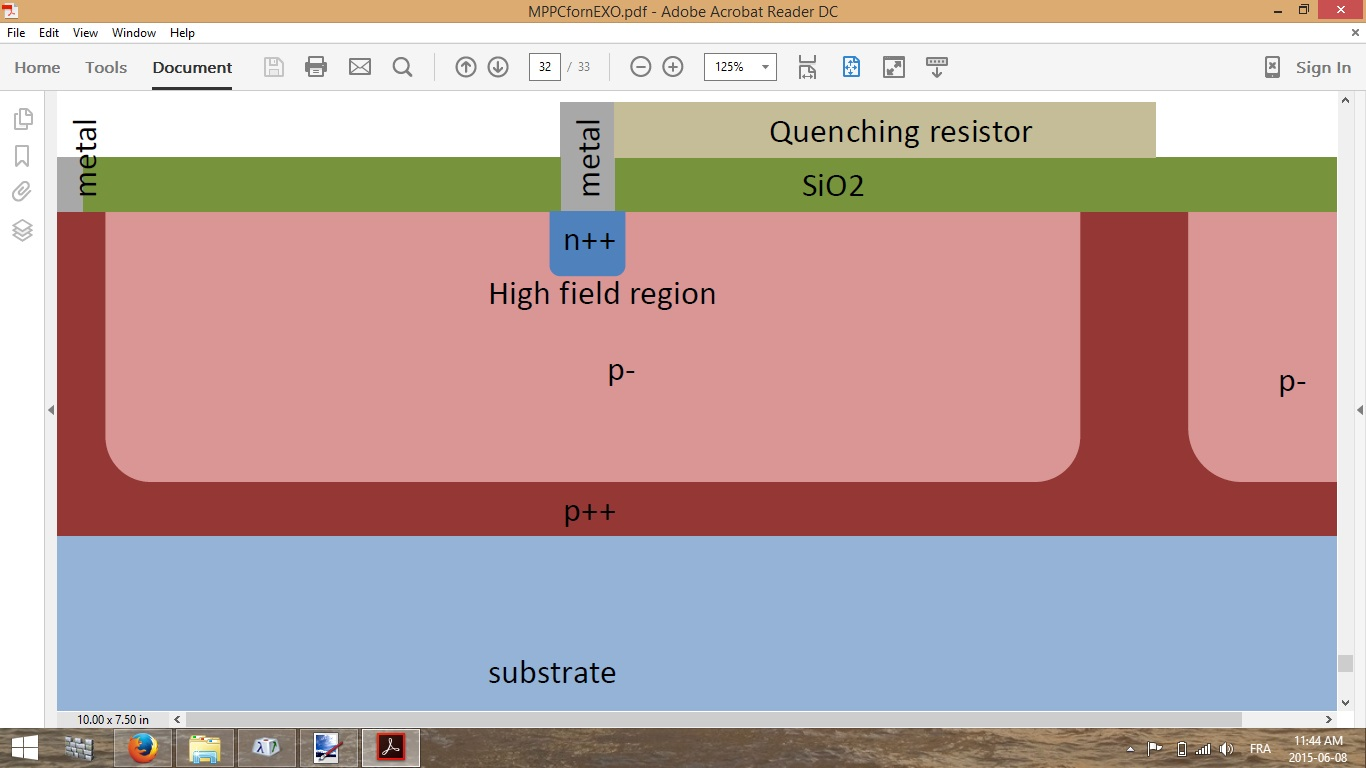
\includegraphics[trim=1.5cm 2cm 5.5cm 3cm, clip=true,totalheight=.4\textwidth]{Pictures/blabla/PN_junction.jpg}%trim=10cm 4cm 1cm 12cm, clip=true, 
  \caption{Details of a pixel of a SiPM.}
  \label{fig:PN_junction}
  \end{figure}
  
  This reference could remind the reader how works a PN junction.
  
  \subsubsection{Principe of avalanche multplication}
  
  The principle of an APD is based on the conversion of the energy of photon into free charge carriers (electrons and 
  holes)in the 
  and their further multiplication via the process of the impact ionisation. 
  \\
  When light (photon) enters a photodiode, electron-hole pairs are generated if 
  the light energy is higher than the band gap energy. Light energy (electron-volt (ev)) and wavelenght lambda (nm)
  are in relationship as shown in equation (number) below. 
  
  \begin{equation}
   e= 123/lamba
  \end{equation}
  
  A reverse volatge (or bias voltage) is applied to each opposite sides (cathode and anode) of a PN junction. The reverse voltage applied on that PN junction
  is higher than the Breakdwon Voltage (BV) of that 
  APD: this is the Geiger mode\footnote{by opposition to the normal mode where the voltage applied to a PN junction is 
  lower than the breakdown voltage}. 
  Also this reverse voltage create an electric field developped across the PN junction.\\
  When an electron-hole pair is generated in the depletion layer of a photodiode 
  the electrons (negative charge) drift towards the N+ (where the anode is) side while the holes drift towards the P+(where the cathode is)
  side due to the electric field. 
  \\
  
  The drift speed of these electron-pairs or carriers depends on the electric field strength. To a certain speed
  the carriers collide with the atoms (called crystal lattice) of the structure. But if the reverse voltage is increased even further, 
  some of the carriers which escaped primary collision with the crystal lattice will have a great energy.\\
  When they collide later with the crystal lattice, they wil generate other electron-hole pairs. This physical phenomen is called ionization:
  an electron or a hoole with high cinetical energy ionize the matter by triggering other electron-hole pairs. 
  By the end an avalanche phenomena is observed inside the avalanche region of a PN junction:
  
  \centering
  \begin{figure}[!hbtp]  
    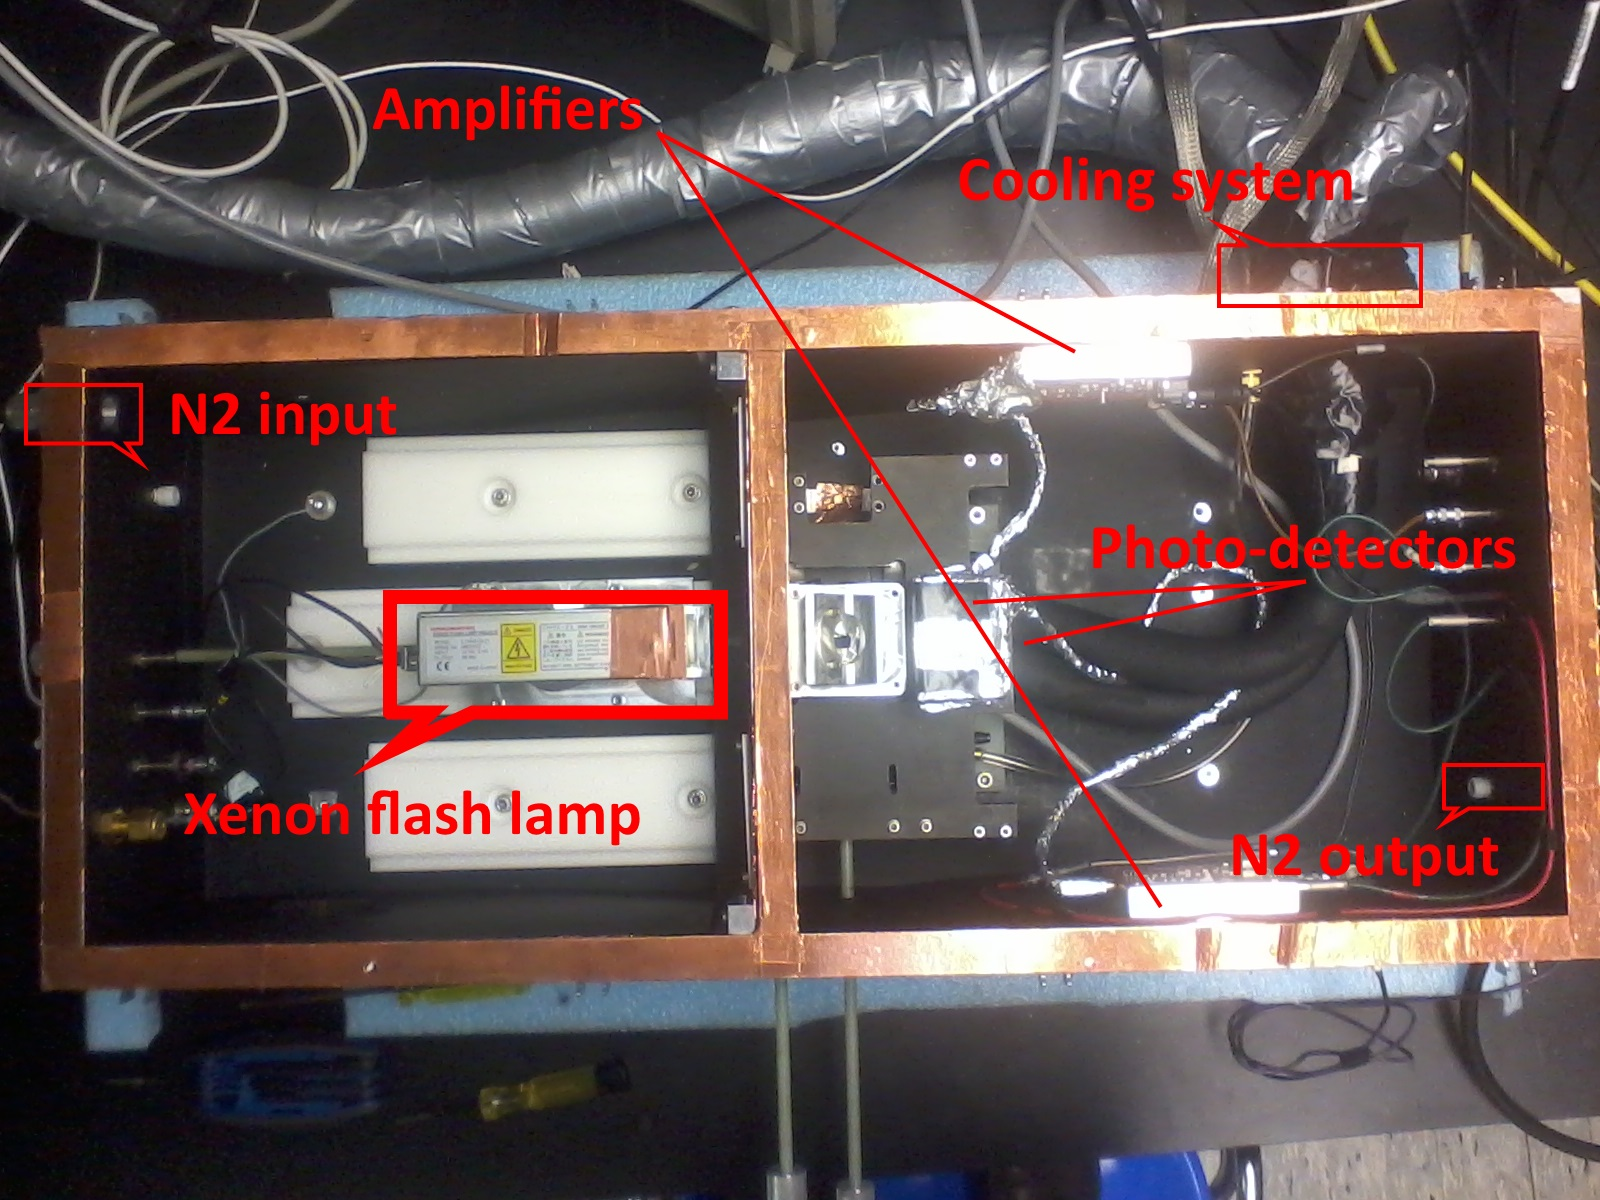
\includegraphics[totalheight=.35\textwidth,trim=0cm 7cm 0cm 2.5cm, clip=true,]{../Pictures/blabla/box.jpg}
    \caption{A photon triggers an avalanche of electron-hole pairs inside the PN junction.}
    \label{fig:avalanche}
  \end{figure}
  
  The electrons of that avalanche phenomena are collected on the anode. The resulting current is used to plot the  pluse shape. 
  To control the avalanche and so the corresponding current, a resistor is set in serie with an PN junction\footnote{The avalanche 
  is limited by the buildup of a limiting space charge in the depletion layer (p-) which decreases the field.}. 
  When the avalanche current flows through the resistor, the bias voltage applied to the junction drops below the breakdown voltage. 
  This quenches the avalanche; thus, the current decreases to zero, and the reverse voltage across the PN junction increases again above 
  its BV.
  \\
  
  The pixel is then ready to detect the arrival of a new photon.\\
  The avalanche current gives a pulse shape obeserved on the screen of an oscilloscope\ref{fig}.
  
  
  %about the gain, simple approximation speak about it ???? not now but in the gain stuff inside the corpus if room therwise in the 
  %appendix
  %Gain: The gain of the SiPM determines the charge which is produced by a single avalanche.
  %In good approximation, the gain depends linearly on the pixel capacitance C pixel and the
  %applied over-voltage V over which is defined as the difference of the bias voltage and the
  %breakdown voltage:
  %C pixel
  %C pixel
  %G = ·V over =   · (V bias −V break ).  (2.1)  q e  q e
  %Here, q e is the elementary charge and C pixel the pixel capacitance.

  \subsection{The three issues of operating SiPM.} 
  
  Such ideal picture is strongly modified by the occurrence of phenomena leading to dark current, afterpulsing effects and crootalk: 
  
  \begin{figure}[!hbtp]
  \centering
  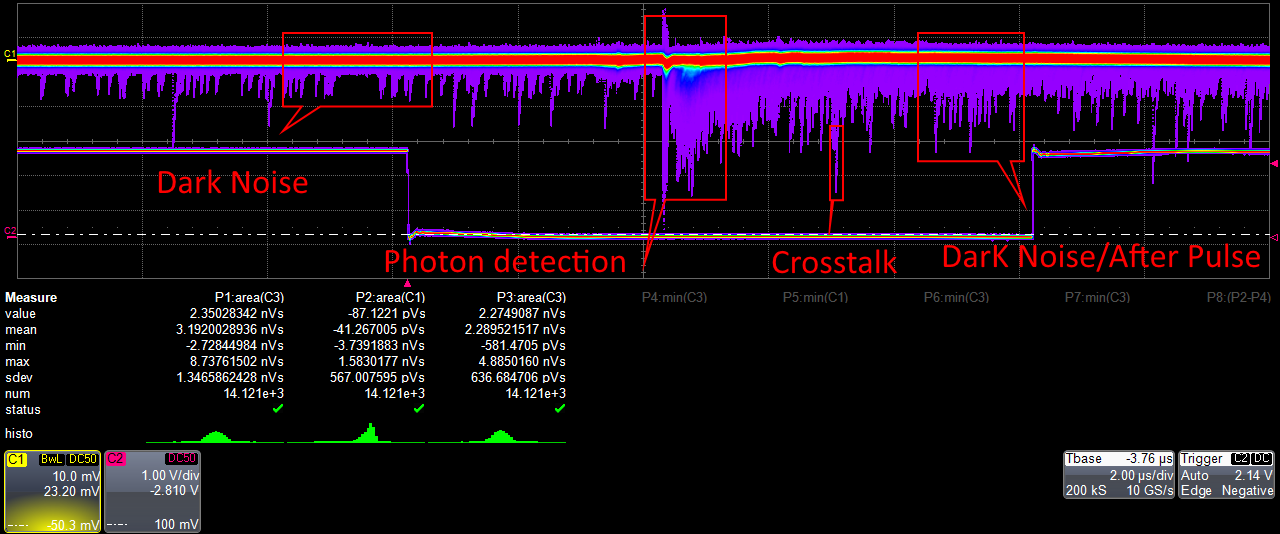
\includegraphics[totalheight=0.22\textwidth,trim=0cm 6.5cm 0cm 0cm, clip=true]{Pictures/blabla/DN_AP_CT_1.png}
  \caption{Dark noise, after-pulse and croos-talk}
  \label{fig:DN_AP_CT}
  \end{figure}
  
  \subsubsection{Dark Noise.}
  
  One of the main source of noise limiting APDs' performance is the dark noise rate.\\
  Elctron-hole pairs are generated thermally in the depletion layer. Due the reversed bias voltage applied on the PN junction, 
  the avalanche phenomena occurs.
  Unfortunately it is not possible to make the difference between avalanche triggered by a photon and avalanche triggered by hot carriers.
  The figure below prove/shows that evidence:
  
  \begin{figure}[!hbtp]
  \centering
  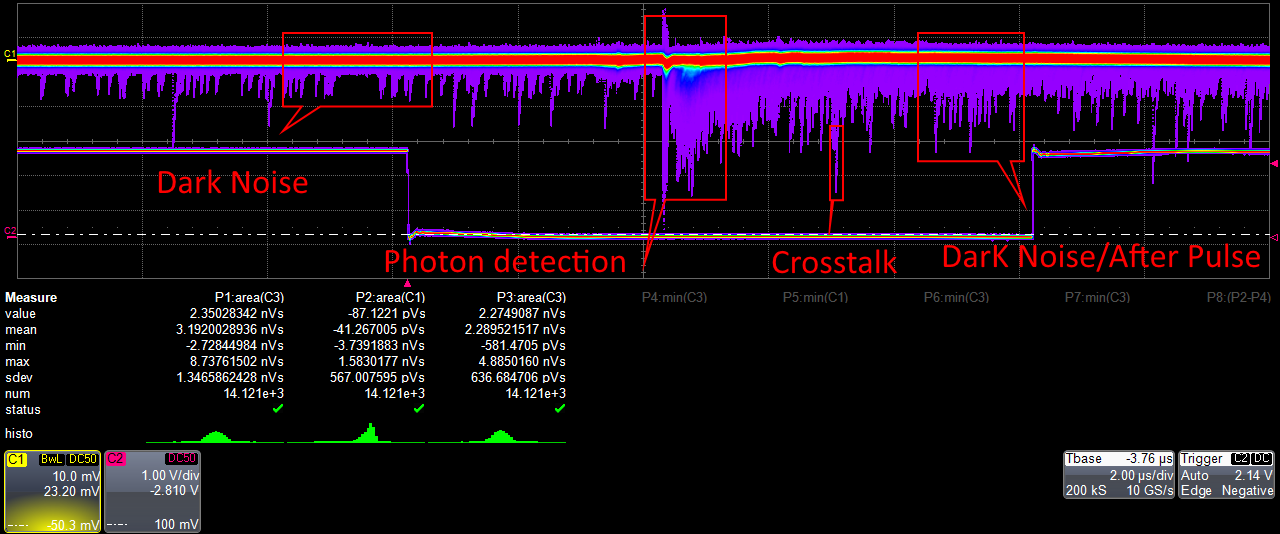
\includegraphics[totalheight=0.22\textwidth,trim=0cm 6.5cm 0cm 0cm, clip=true]{Pictures/blabla/DN_AP_CT_1.png}
  \caption{Pulse shape due to a photon is exactly the same than pulse shape dur to hot carriers.}
  \label{fig:DN_photon}
  \end{figure}
  
  Dark noise depends only of the structure of the SiPM. The array \ref{appendix} shows that HAMMAMASTU can build SiPM with low dark noise rate. 
  Nevertheless it is possible to decrease the dark noise rate by cooling down the SiPM since darke noise is generated by 
  hot carriers.  
  
  Moreover Dark noise follow a poisson law (to complete).  
  
  \subsubsection{Trapping phenomena: Afterpulsing.}

  Traps may result from damage caused by an implantation of some impurities in the fabrication process. In the depletion layer, 
  deep levels trap some avalanche carriers and release them with 
  a statistical delay. If the delay is greater than the dead time after the previous avalanche pulse, a released carrier can
  re-trigger an avalanche and cause a statistically correlated pulse. These delayed corrolated pulses are known as afterpulse. 
  \\
  
  \begin{figure}[!hbtp]
  \centering
  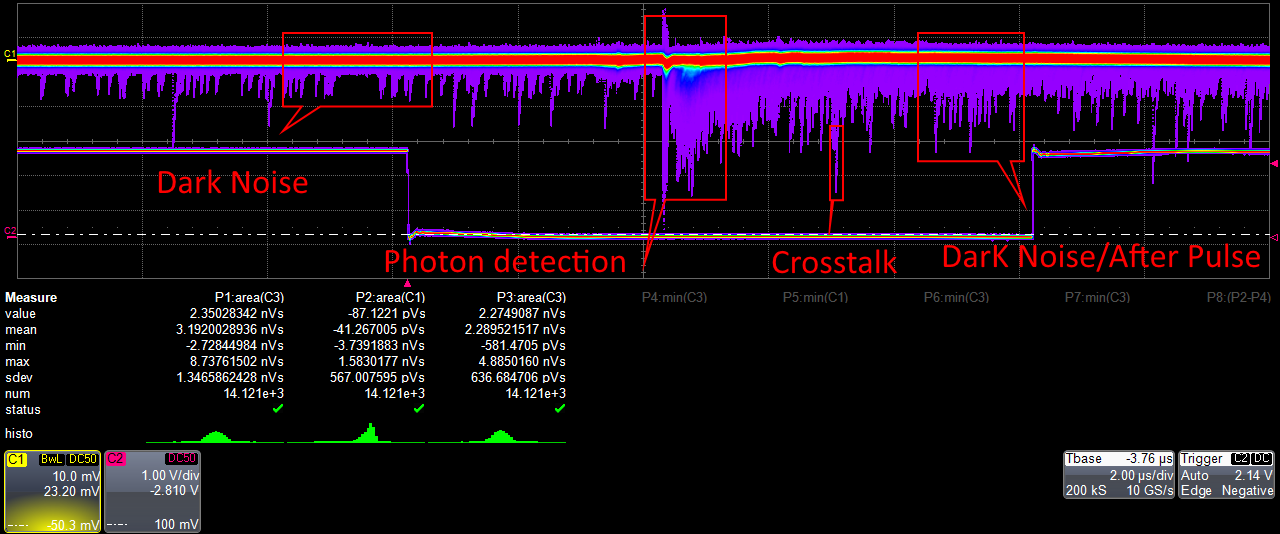
\includegraphics[totalheight=0.22\textwidth,trim=0cm 6.5cm 0cm 0cm, clip=true]{Pictures/blabla/DN_AP_CT_1.png}
  \caption{After pulses are clearly identified with the persistent mode of the oscilloscope.}
  \label{fig:AP}
  \end{figure}
  
  The probability that an afterpulse occurs increases with the reversed bias voltage applied on the SIPM.  A solution to diminish 
  significatively afterpulse effects is 
  to operate at low reversed bias voltage, but at the expense of degrading the photon-detection efficiency (see section). 
    
  After pulse follow a law. 
  
  \subsubsection{Optical crosstalk.}
  
  Hot carriers (e.g., dark noise) in avalanche PN junction has a certain probability to emit photons with energy higher than 1.14 ev (higher than 
  the band gap energy described in section).\\
  Depending on their energy and the location where they are produced, these photons have a certain probability to reach a 
  neighbouring pixel and to produce an additional avalanche. 
  
  \begin{figure}[!hbtp]
  \centering
  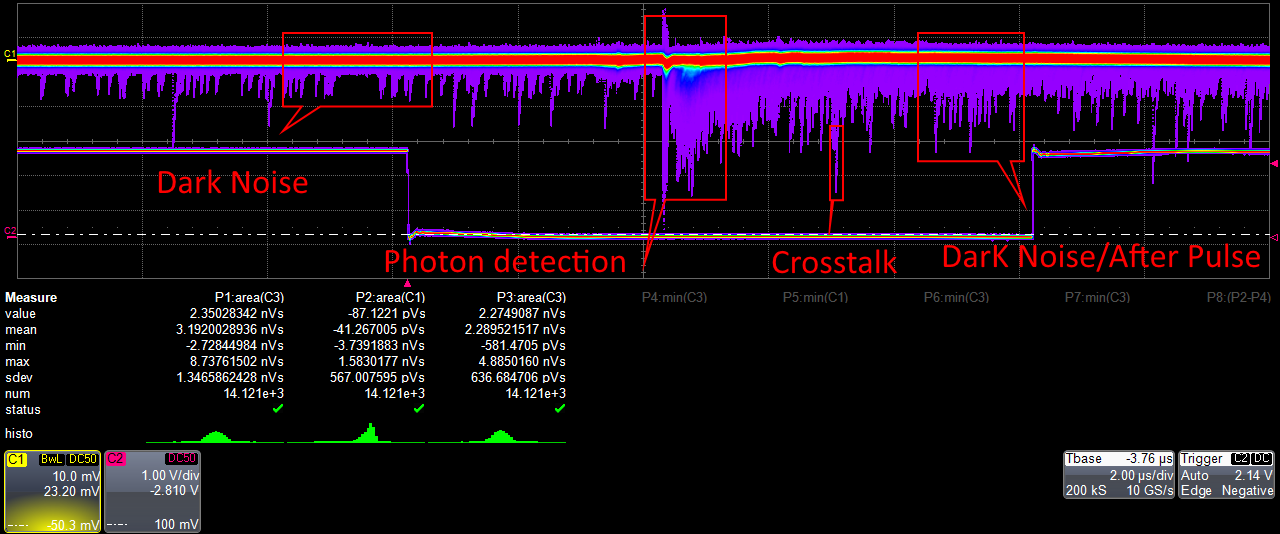
\includegraphics[totalheight=0.22\textwidth,trim=0cm 6.5cm 0cm 0cm, clip=true]{Pictures/blabla/DN_AP_CT_1.png}
  \caption{Photons emit may reach a neighbouring pixel and trigger there an avalanche.}
  \label{fig:CT}
  \end{figure}
  
  So at conditions where only one pixel is expected to be excited simultaneously than its neighbouring pixels, crosstalk results in output 
  pulses with amplitudes twice or several times the amplitude of a single triggered pixel
  \footnote{The section\label{Basic operation} reminds that ``The total output signal is equal to the sum of those from the indidividual 
  pixels firing by photons''.}
  
  A technical solution is to build an optical wall between two pixels (not enough). 
  \\
  
  The probability of observing crosstalk is proportional to the SiPM gain and so to the reversed bias voltage. The same conclusion about the 
  efficiency made in the previous subsection are obeserved for crosstalk. 
  
  The law
  
  
  \section{Encountered issues}  
  
  Before recording waveforms and analysing them I dealed with some issues but mainly with electronic noise.\\
  Light leaks appeared when the \xfl was operating. They can hinder and negate the results of data collection. 
  Two kinds of light leaks have been observed :
  
  \begin{itemize}
   \item Visible light leaks.
   \item Radiofrequency light leaks.   
  \end{itemize}
  
  \subsection{Visible light leaks}
  
  Visble light leaks come from outside of the box or from the \xfl (If ... complete).\\
  This phenomena has mainly an impact on the dark noise rate and on the calculation of the efficiency.
  To avoid visible light from the \xfl, the last one is covered with black box. Also to absorbe photons from such visible light
  walls and lid is covered by matt black absorbing vin.\\
  To avoid light from outside of the box, the whole box was covered with a black tissue. The section \ref{} shows how we check if some
  visible light from outside could reach detectors inside the box. 
  
  \begin{figure}[!hbtp]
  \centering
  \begin{subfigure}{.5\textwidth}
    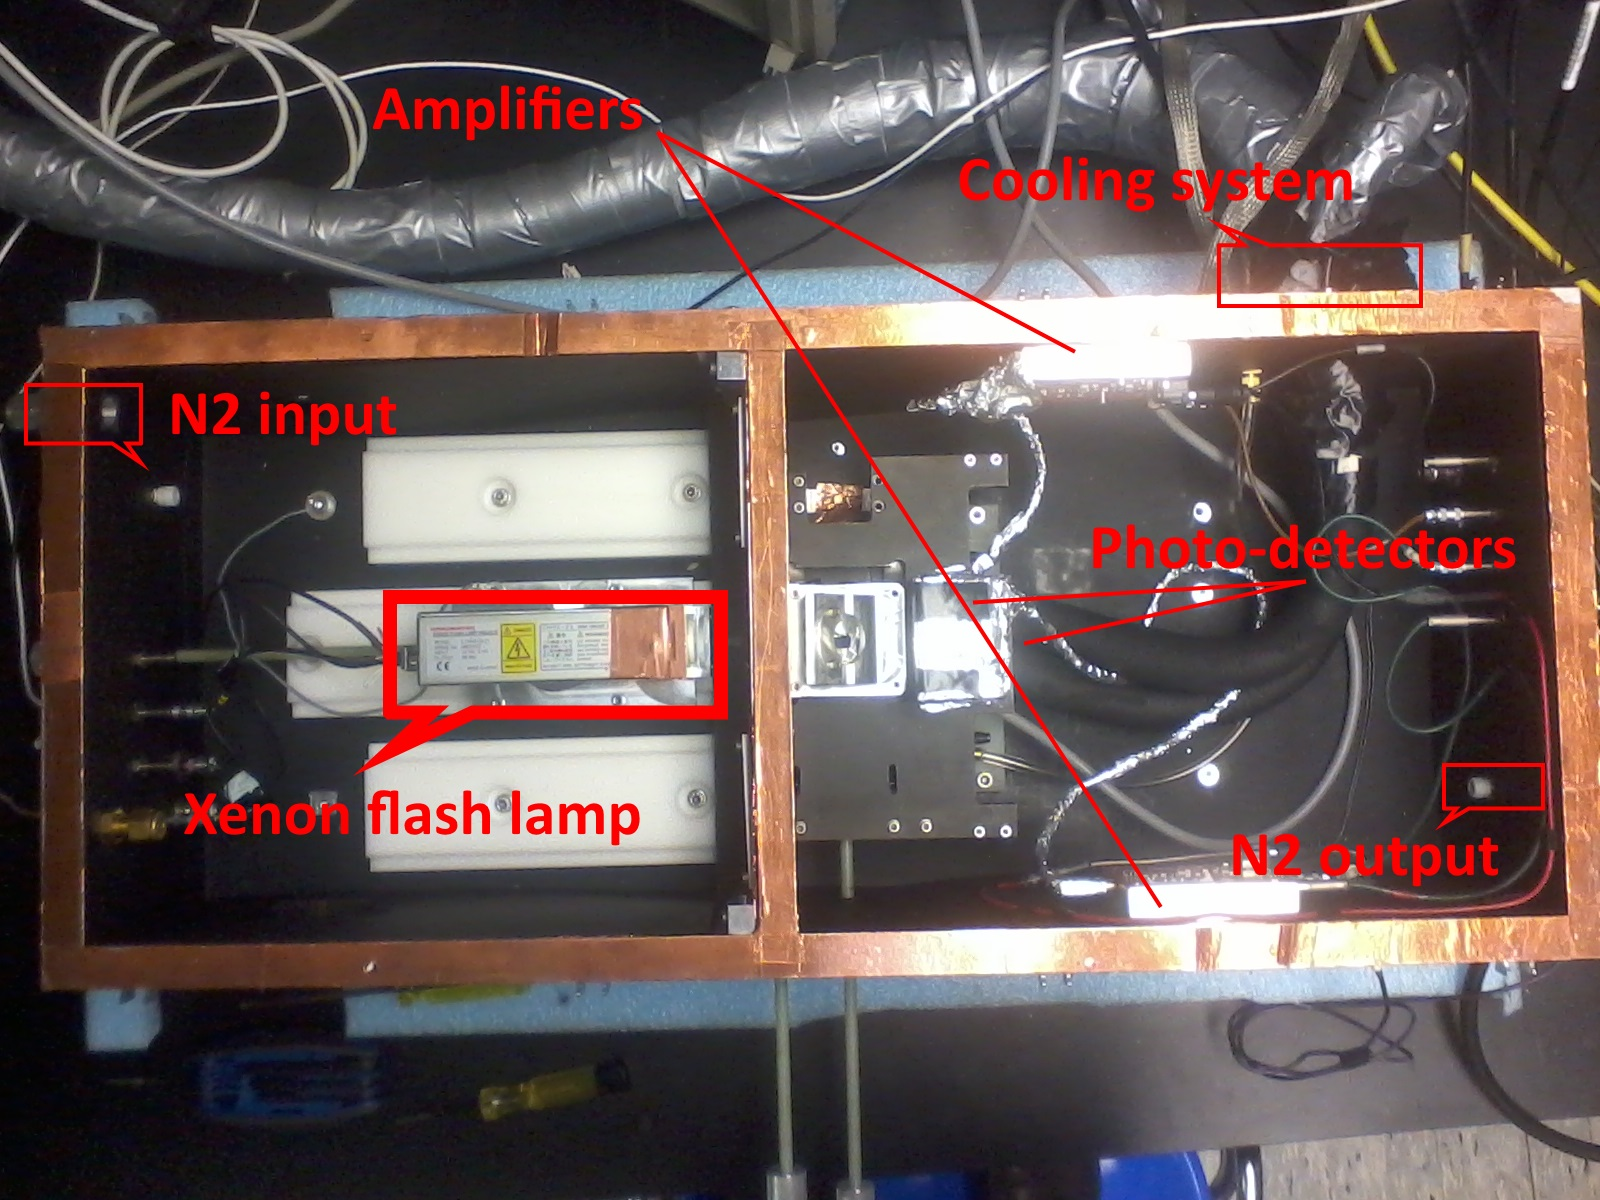
\includegraphics[totalheight=.35\textwidth,trim=0cm 7cm 0cm 2.5cm, clip=true,]{../Pictures/blabla/box.jpg}%trim=10cm 4cm 1cm 12cm, clip=true, 
    \caption{A SiPM from HAMMAMATSU VUV sensitive.}
    \label{fig:SiPM}
  \end{subfigure}%
  \begin{subfigure}{.5\textwidth}
    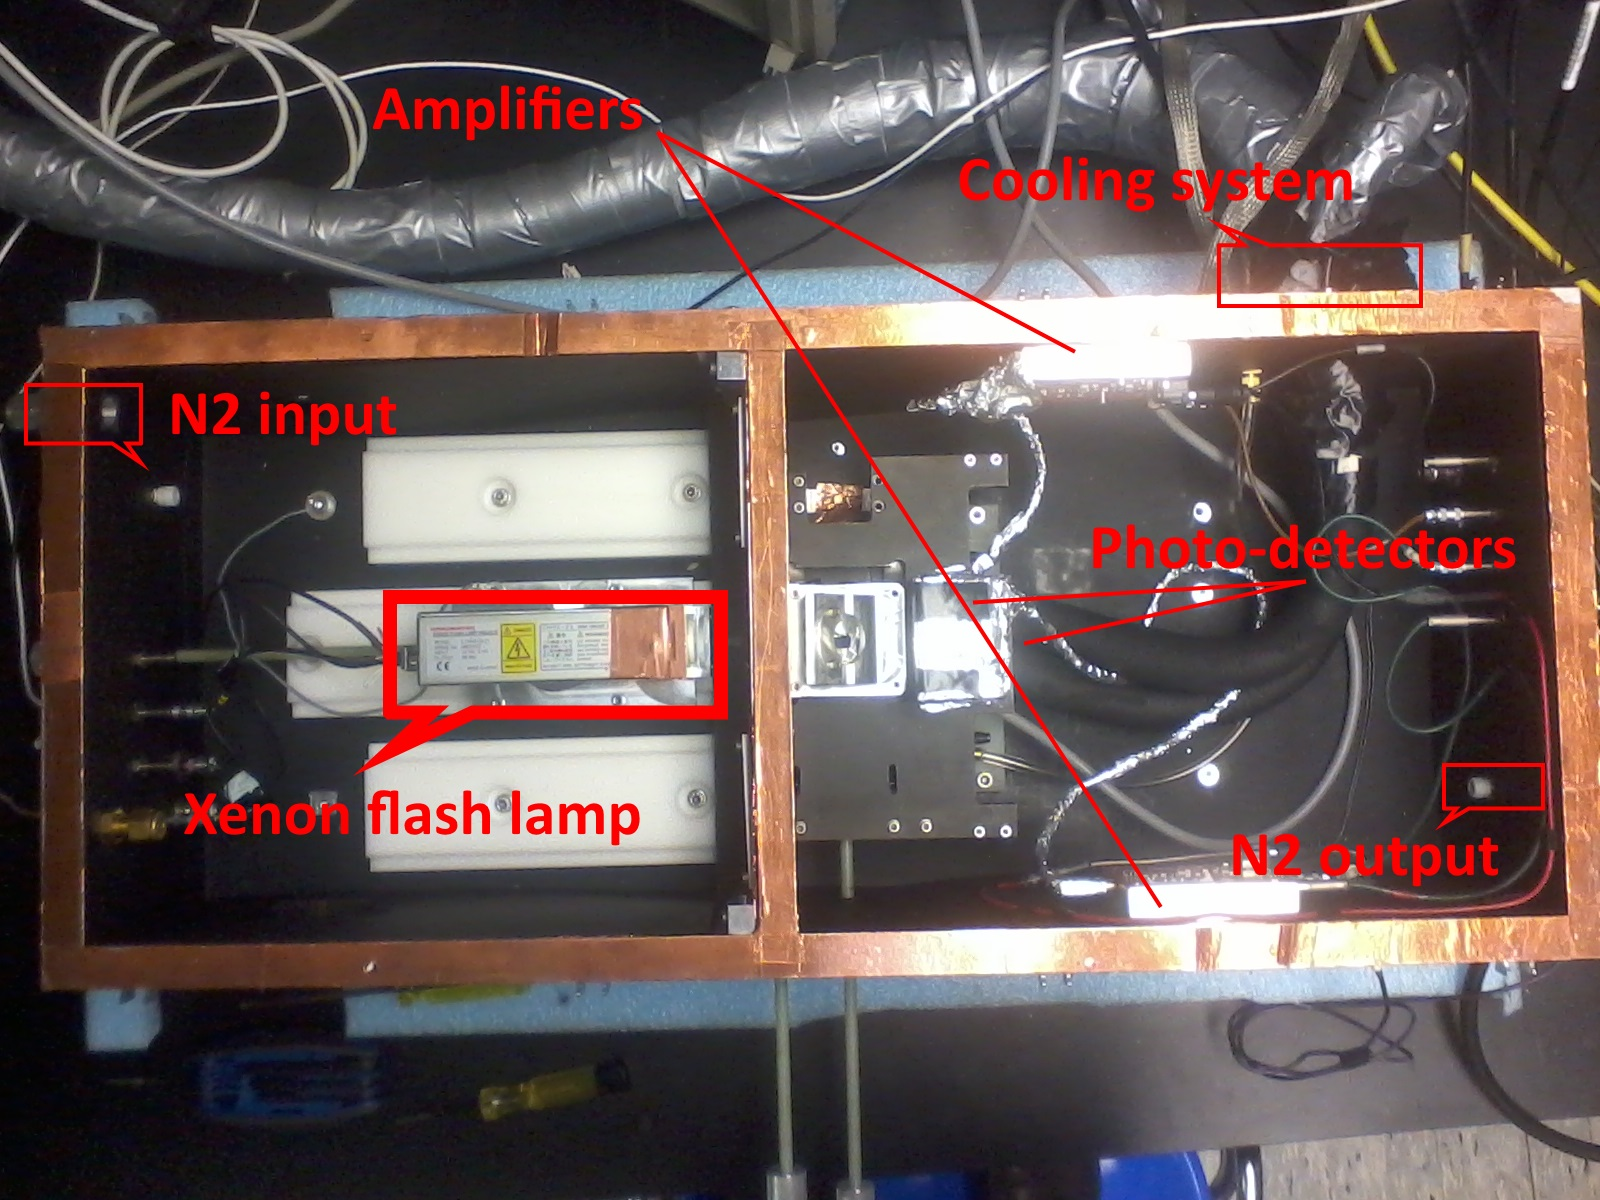
\includegraphics[totalheight=.35\textwidth,trim=0cm 7cm 0cm 2.5cm, clip=true,]{../Pictures/blabla/box.jpg}
    \caption{Equivalent circuit.}
    \label{fig:electrical_circuit}
  \end{subfigure}
  \end{figure}
  
  \subsection{Radiofrequency light leaks.}
  
  Radio frequency light leaks result in electromagnetic noise on the signals from the detectors.\\  
  Radiofrequency noise occured when the \xfl was triggered by a square wave pulse generator. Too much readiofrequency noise disturbed 
  the signals of the photodetectors. The figure \ref{} shows clearly that electronic noise covers, deformes or amplifies pulse shapes.
  
  \begin{figure}[!hbtp]
  \centering
    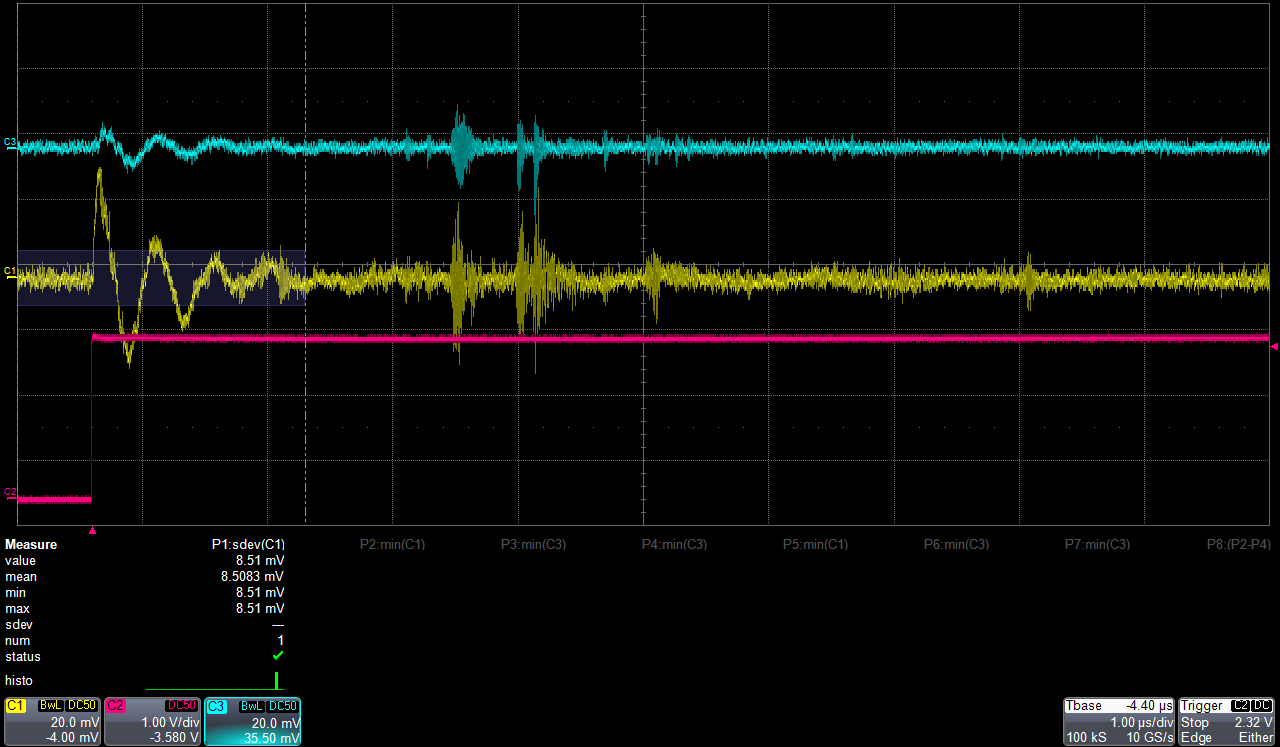
\includegraphics[totalheight=0.4\textwidth,trim=0cm 5.5cm 0cm 0cm, clip=true]{Pictures/lamp_noise_apr17_2.png}
  \label{fig:noise_signal}
  \end{figure}
  
  \subsubsection{Sources of electromagnetic noise.}
  
  We noticed that electronic noise came from electromagnetic sources. So

  \begin{itemize}
  \item Some devices were not grounded. The signal from the photodetector oscillate\ref{fig:noise_signal}
  ~\ref{fig:signal_with_noise}.
  \item When the \xfl was working it was creating some radio waves propagating through the air and which were then transmitted to any piece of conductive metal of the 
  box. The consequences were : 
    \begin{itemize}
    \item The aluminium lid of the box conducted everywhere the electric field of these radio waves, which disturbed the amplifiers.
    \item Each detector could feel these radio waves and the signal got worst.
    \item The metal divider acted as a transmitter and the piece of metal of the signal wires connected to the amplifiers acted as antenna.
    \end{itemize}
  \end{itemize}
  
  \subsubsection{Three main solutions.}
  
  The first solution was to create a ground point on which all devices - especially the square wave pulse generator - were connected with the same wire 
  (to avoid ground loops). In that way, the oscillations of ~\ref{fig:comparaison} were removed. 
  
  \paragraph{\underline{\emph{Isolate the lid from the box.}}}
  
  As it was described above, the electric field from the radio waves propagates through the entire lid. When the box was closed it disturbed the working 
  amplifiers. The solution was to isolate the lid from the box by adding black tape and to guide the electric field with copper on the edge of the lid
  to the ground point.

  \paragraph{\underline{\emph{Isolate the \xfl.}}}
  
  As the \xfl creates radio waves, we decided to isolate it by building a faraday cage around it. We added a thick piece of metal to absorb radio waves 
  and we covered this first part of the box with aluminium foil. In that way the electric field propagates through the aluminium foil to the edge of the top
  box to the ground point. 

  \paragraph{\underline{\emph{Isolate the photo-detectors and the amplifiers.}}}
  
  As the bottom and the top detector seems to capture radio waves, two faraday cages were created to protect them.
  
  This picture below could summarize our work (yellow signal is the bottom photodetector and the blue one is on the top):
 
  \begin{figure}[!hbtp]
  \begin{minipage}[t,High electronic noise level.]{0.49\linewidth}
    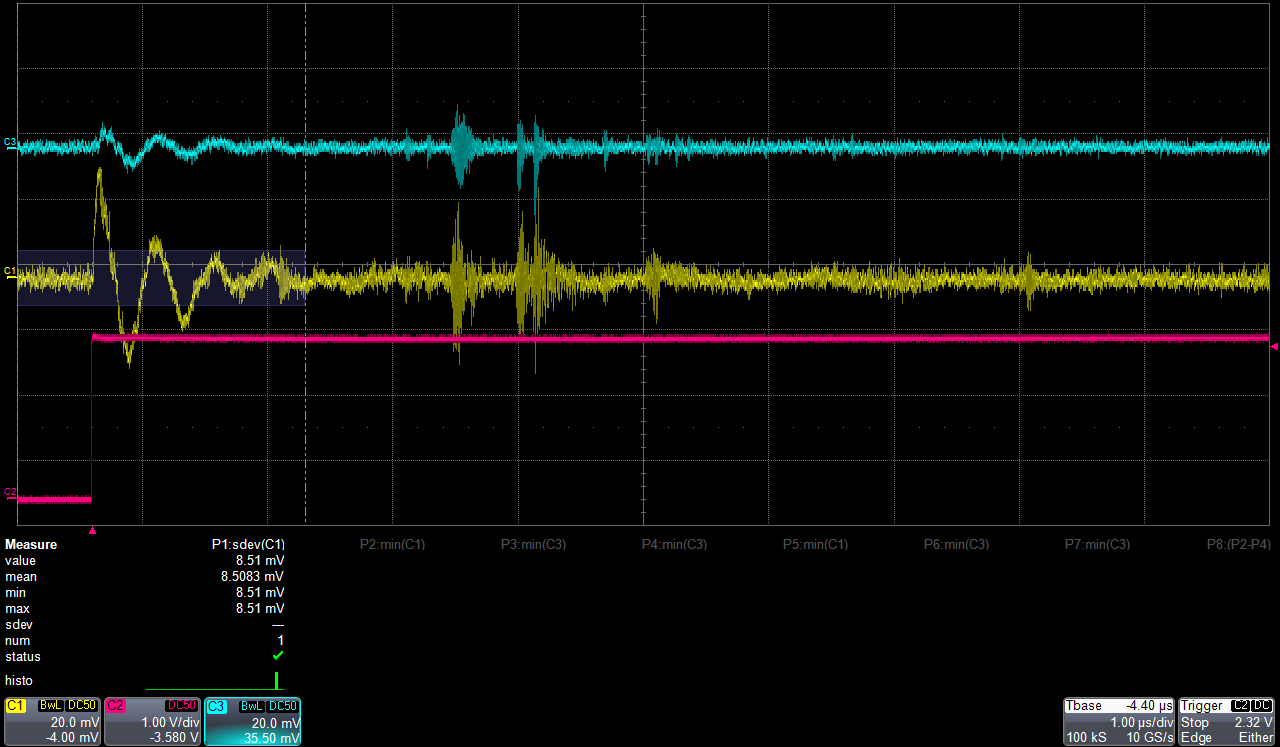
\includegraphics[totalheight=0.4\textwidth,trim=0cm 5.5cm 0cm 0cm, clip=true]{Pictures/lamp_noise_apr17_2.png}
    %\centering{\caption{Noisy signals.}}
    %\label{fig:Noisy_signals}
  \end{minipage}
  \quad
  \begin{minipage}[t,Low electronic noise level.]{0.49\linewidth}
    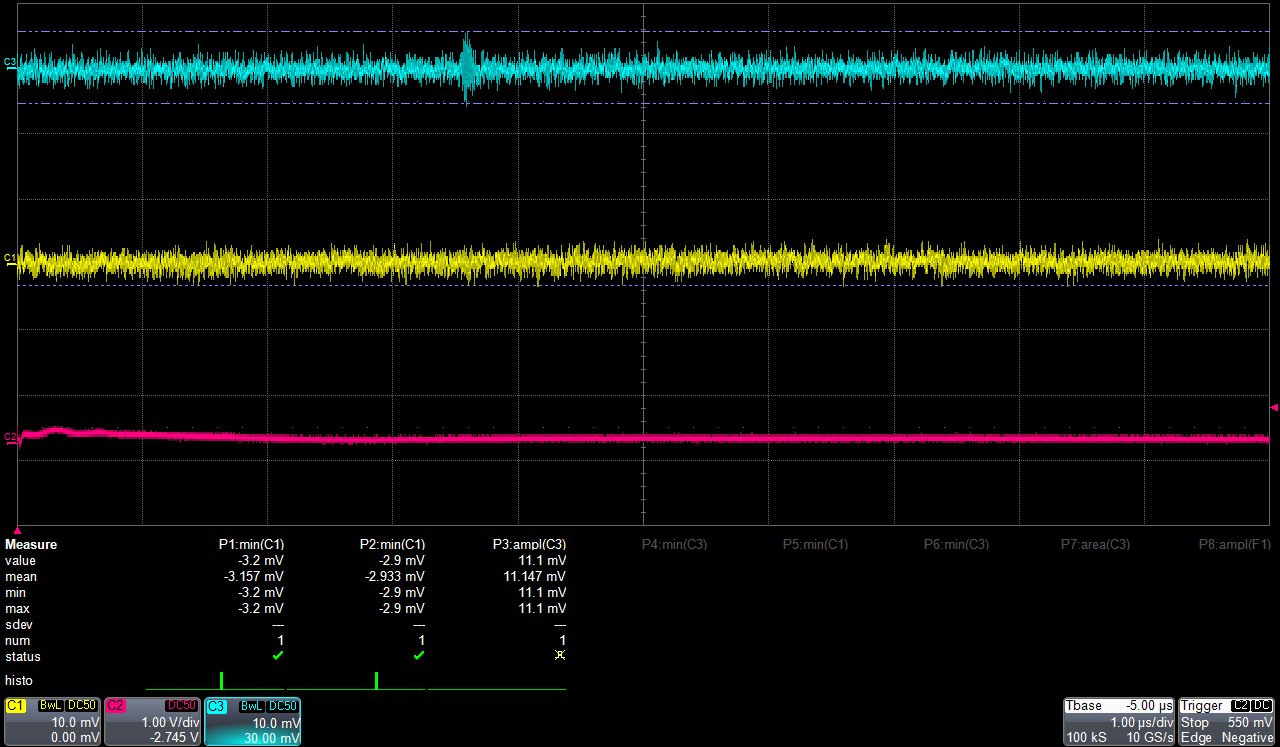
\includegraphics[totalheight=0.4\textwidth,trim=0cm 5.5cm 0cm 0cm, clip=true]{Pictures/good_elec_noise.png}
    %\centering{\caption{The electronic noisehas dispeared.}}
    %\label{fig:good_signals}
  \end{minipage}
  \caption{The noise level before (left) and after (right) solving the issues.}
  \label{fig:comparaison}
  \end{figure}
  
  
  %\begin{figure}[!hbtp]{0.49\linewidth}
  %\centering
  %\subfigure[High electronic noise level.]{
  %  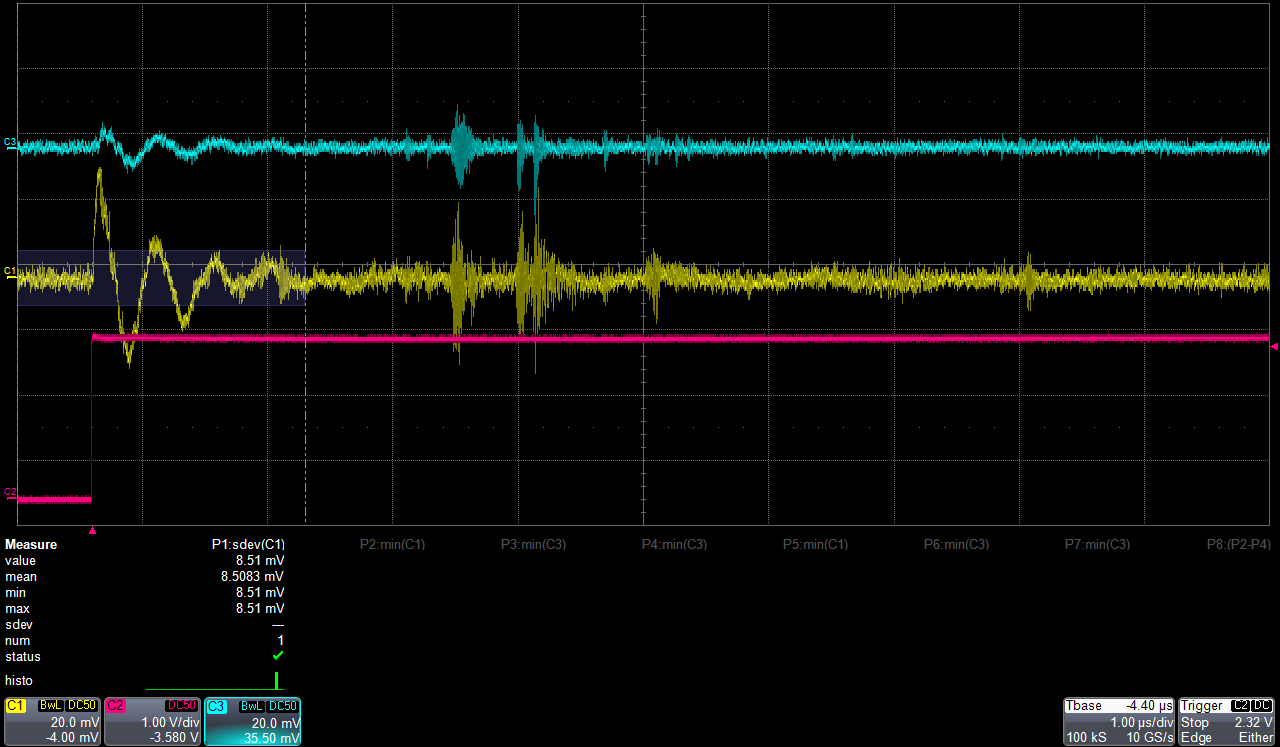
\includegraphics[totalheight=0.4\textwidth,trim=0cm 5.5cm 0cm 0cm, clip=true]{Pictures/lamp_noise_apr17_2.png}
   % \label{fig:noise_signal}}
  %\quad
  %\subfigure[Good The electronic noisehas dispeared.]{%
    %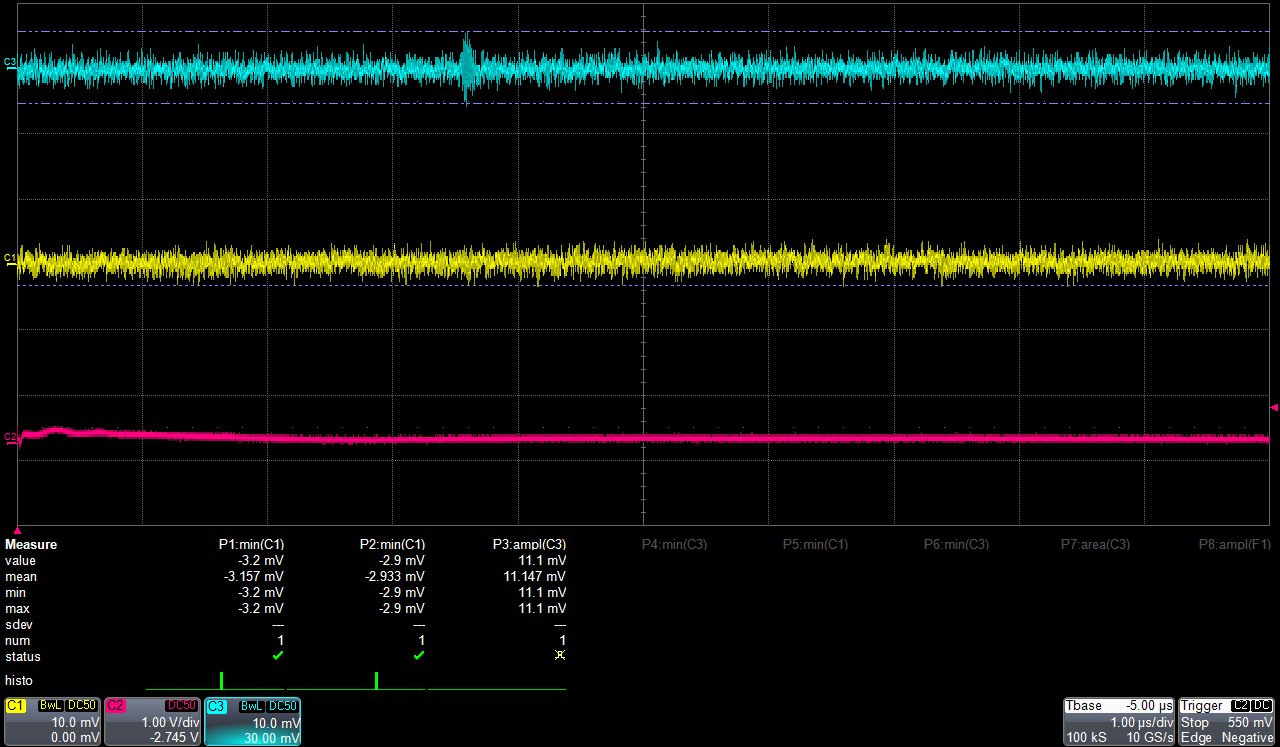
\includegraphics[totalheight=0.4\textwidth,trim=0cm 5.5cm 0cm 0cm, clip=true]{Pictures/good_elec_noise.png}
    %\label{fig:good_signal}}
 % \caption{The noise level before (left) and after (right) solving the issues.}
 % \label{fig:comparaison}
 % \end{figure}
  
  A SiPM, placed on the top, was used as a reference. It let us check if the light remained constant when we characterized a MEG MPPC and a VUV3 SiPM at 
  $-100^\circ$C.
  
  
  \section{DN rate and After Pulse}\label{DN}
  
  \subsection{recoveries time and amplitude/distribution of tim ..}
  
  As mentioned earlier, the distribution of the timing difference between consecutive pulses is used to measure the dark noise and 
  after-pulsing rates. The starting pulses are required to correspond to the oscilloscope trigger in order to properly
  account for the oscilloscope dead time. The starting pulses are also required to correspond to single pixel avalanches
  (i.e. triggers with cross-talk are excluded) in order to measure the after-pulsing rate generated by a single parent avalanche.
  On the other hand, the second pulse can have any amplitude (above the noise). 
  
  Fig pulse amplitude vs time newt pulse shows the amplitude of the second pulse as a function of the time difference with the trigger
  pulse. 
  The main band (the first one with fitting function) at ∼40 mV corresponds to single pixel avalanches. 
  Cross-talk yields pulses with amplitudes two, three, or more times larger. 
  
  10³ ns = 1 µs; lamp send pulse of 10 µs -> 10⁴ ns.
  
  There is no correlation between time and amplitude except below 100 ns where a drop below the 40 mV value is clearly visible. 
  Physically inside the  photodector, after an avalanche the voltage across the diode indeed recovers with a time constant 
  given by the product of the pixel capacitance and quenching resistance. The pulses that do not have lower amplitude even
  though they occurred within the recovery time scale must
  come from different pixels. It is likely that these pulses are
  delayed cross-talk, the seed charge carrier being created by
  photons from the parent avalanche subsequently diffusing to
  a neighboring pixel. This feature is also clearly visible for the VUV3. 
  
  The timing distributions are shown in Fig. 15 including the function that best fits the data. Each step on a log-log plot
  corresponds to a distinct exponential time dependence. The last step corresponds to distribution of dark pulses. It is clearly
  visible for all 3 devices. 
  
  The difference is striking because the FBK-2013 SiPMs are 9 times smaller in area than the VUV3. check this for our experience. 
  
  dark noise rate is an order of magnitude too high
  
  after pulse : After-pulsing rates were also extracted by fitting the distributions
  the total after-pulsing rate and the after-pulsing rate within the first 10 μs that is relevant for our application
  exceeds the specification of 20% for the combined rate of cross-talk and after-pulsing. 
  
  expect limit the number of correlated pulses (cross-talk and after pulse) to less than 0.2 per parent pulse.
  
  
  
  
  
  The darknoise rate is the signature of each device. So to know this signature let us know to compare different devices between them. 
   
  \subsection{methodology for DN and AP: theoriticl calculation and how to act on the setup}
  
  One of the main source of noise limiting the SiPM performance is the dark noise rate, which mainly originates from the electron 
  created thermally in the depletion layer (p-) \ref{figure}. These carriers trigger avalanches exactly as if the pixel would have been fired.
  \\
  To calculat the DN rate, the goal is to count the number of time the screen of the scope
  displays on pulse (by opposition at two pulse detected on the same time \ref{section}). So a simple idea is 
  to record the minimum of of pulses on the dark region \footnote{see ection/figure}. It is quiet easy to understand
  that we have to focus on the dark region only. Indeed the light region match one PE peak match with the detection of one photon-electron send from
  the lamp bu also corresond/reflect the DN/match with the detection of one PE from DN. So the light region of the scope do not let us determine for shure from where comes 
  this pulse. So to avoid to be confused we have to focuse on the dark region only. 
  \\
  
  On the scope we trigger one the lamp.then we recorded the minium of pulses of the dark region and plot
  them on an histogram. The first PE peak match with the detection of zeroPE. The second with detection of one PE etc. 
  
  \subsection{results : plot}
  
  The historgam of fig (section PE) is used for DN..
  
  nEXO experiment requires that at -100C, the DN rate should be less than 50HZ/mm². 
  It is interesting to observe tat the DN rate decrease with the temeperature. 
  
  \begin{figure}[!hbtp]
  \centering
  \includegraphics[totalheight=0.4\textwidth,trim=1.8cm 1cm 5.5cm 3cm, clip=true]{Pictures/Pictures_MEG/DN.png}
  \centering{\caption{light region.}}
  \label{fig:pulse_shape}
  \end{figure}
  
  \subsection{analyse : pont entre méthodoligie et solution }
  
  \paragraph{factor which could influence DN}
  
  The DN depends of each device. The DN depend only of the temperature as it was described above. 
  
  \paragraph{}
  
  the ref and the annexe could givemore detail about the theoritical calculation of DN. 
  
  \begin{equation}
    P_{D0} =  exp(-<DN>) \iff <DN> = -ln(P_{D0}).
  \end{equation}
  
  The DN follows the poisson law. That why in the histogram we inegrate zero pe. For a number of waveform constant/
  for the same total number of waveform, when the temperature decrease, the DN decrease. So the number pe upper than the detection
  of one PE decrease also \ref{see part below} while the number of zero pe increase. 
  According to the equation above, Po increase and so DN decrease.   
  
  \paragraphe{conclusion}
  
  Compared to the MEG SiPM, the VUV3 is a good quandidat for nEXO.  
  
  \section{CT}
  
  They unfortunately all exceed 20%, 
  which is our upper limit for the correlated avalanche probability that includes cross-talk and after-pulsing.
  
  Hot carriers in avalanche p-n junction emit photons even in the visible range \footnote{see section}. Thus, 
  during the avalanche breakdown, a photodiode operating in Geiger mode may emit a few photons. 
  The photons emitted will be detected by neighboring pixels despite an optical wall between two pixels \footnote{see picture annexe}. 
  \\
  
  It is quiet esay to identify crosstalk on the screen of the scope \footenote{see section, gif orput figure}. 
  When the height of a peak is double compare to its neighbor, this peak is a cross talk. Physically that means that two avalanche appears and end 
  on the same time : one comes from the photon coming from a neighboring pixel and the other one comes from the detection of a photon or 
  reflect dark noise. 
  
  \subsection{methodology for CT: theoriticl calculation and how to act on the setup}
  
  When we trigger on the lamp, the minium for each waveform recorded is taken in account/ is recorded. Then we construct an histogram 
  \footnote{see section} where the first peak of the histogram match with zero peak. The second peak match with the detection of a photon or 
  comes from dark noise. The third peak match with the detection of two photon on the same time, ie crosstalk.\\
  The screen on the scope displays gaussian noise for the case, a single peak for the second and a double higher peak for the third. 
  
  So to analyse crosstalk, the idea is to eradicate the first peak of our previous histogram. the goal
  is to obtain an histogram where the first peak match with the detection of 
  one photon while the second peak of this futur histogram match with the detection of two photon which appear on the 
  same time.\\
  That means that instead of triggering the scope when the lamp send flash we have to trigger when the scope displays
  one peak corresponding to the detection of one photon or coming from dark noise. 
  So as it has been seen previously\footnote{see section} that the DN is always appearing, we triggered on the detector. 
  image. 
  
  \paragraphe{method}
  1 range of time of 2ns(1ns before and 1ns after}\\
  2 set a threshold at 3.5 times the baseline to record a minimum amplitude\\
  3 Set data in a table and plot an histogram
  4 Integrate the first peak and divide by the totale number f waveform (or integrate the histogram from the beginning of the first peak)
    
  \subsection{results : plot}
  
  Here is an histogram of CT for VUV3 @ -100C. The first peak correspond to the detection of one photo-electron, 
  the second one to the detection of two photo-electron etc...
  
  \begin{figure}[!hbtp]
  \centering
  \includegraphics[totalheight=0.4\textwidth,trim=1.8cm 1cm 5.5cm 3cm, clip=true]{Pictures/Pictures_MEG/CT_histrogram.png}
  \centering{\caption{Hitogram coming from analysing crosstalk for the VUV3 SiPM @ -100C. }}
  \label{fig:CT_hitogram}
  \end{figure}
  
  The array \ref{see above} describ some device we test. The most intrinsting devices are the MEG SiPM and 
  the VUV3 SiPM both of them from Hammatsu. 
  
  \begin{figure}[!hbtp]
  \centering
  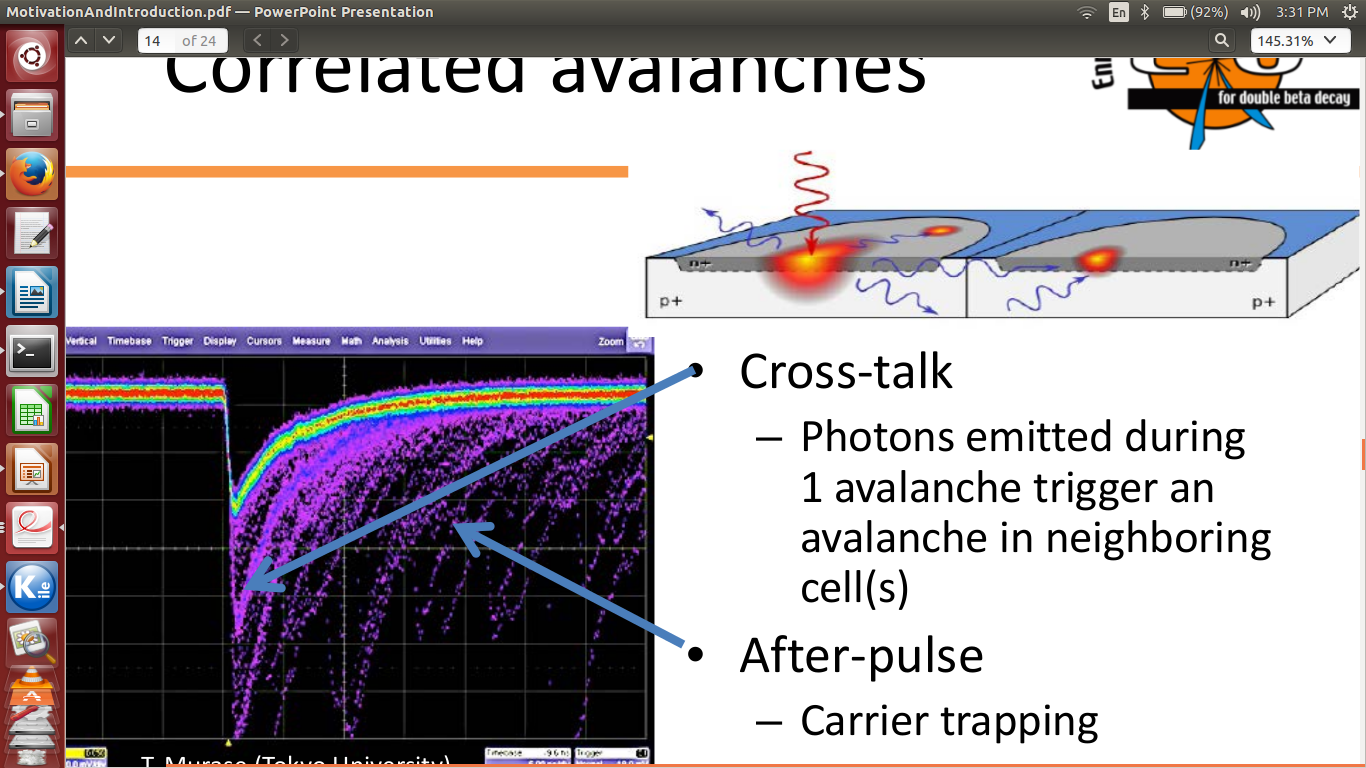
\includegraphics[totalheight=0.4\textwidth,trim=1.8cm 1cm 5.5cm 3cm, clip=true]{Pictures/Pictures_MEG/CT.png}
  \centering{\caption{Crosstalk for the VUV3 SiPM (red) and for the MEG MPPC (blue).}}
  \label{fig:CT}
  \end{figure}
  
  The VUV3 SIPM is quiet interesting because it let us go up to 6/7 OV before reaching the limit of 0.2 per parents
  pulse set for nEXO experiment. 
  
  \subsection{analyse : pont entre méthodoligie et solution }
  
  \paragraphe{factor wich could influence CT}
  
  CT depend only of temperature, light leak (we don't use the lamp since we trigger on the detecor \ref{section}/above}
  and electronic nois. 
  The temperature was not an issue because the cooling system let us check that the temperature reminf constant
  over time (variation of 1 deg maxi). The only issue was with light leak.\\
  Photons from light outside of the box are catched/detected by the detector. The number of one pulse increase and so t
  the probability that crosstalk appear increases also \ref{section}. 
  To prevent light from outside entering inside the box, the box was covered with two black blanked/tissues and the light of t
  the clean room was off. 
  A test \ref{} was made to see the impact of light from outside of the box:
  
  \paragarphe{fitting}
  
  the ref{biblio} let us fit the function. The crosstalk could be calculated quiet easly assuming that law 
  Ct = -ln(P0-dark/total). 
  This seems quiet wierd beacause instead of integrating the second PE peak of the histogram \ref{fig} 
  we count the number of time that on PE appear. 
  But as it was descrived previously \ref{}, the crosstalk increase with the voltage. 
  So with the number of total waveform, the second PE peak increase but the first PE peak decrease. So the PO of the 
  equation decrease and so the CT increase.  
  
  \paragarphe{conclusion}
  
  The VUV3 SiPM seems to be a a good candidat for nEXO. 
  
  \section{PE}\label{section:PE}
  
  Measuring the efficiency of the SiPM we tested is one of the most important test to do to characterize them. unfortunately we failed. 
  Several experiment described in such papers \ref{} have already measure the effiency for SiPM but not in the experiemental conditions
  of nEXO : wavelenght of light at 175 nm and at -100C. 
  
  \subsection{methodology for PE: theoriticl calculation and how to act on the setup}
  
  \paragraphe{theoritical calculation}
  
  Some references \ref{biblio} help to calculate theoritically the efficiency. Here is the equation we used : 
  
  So the average efficiency - \(<PE>\) - of a detector is defined with this relation below: 
  \\
  
  The probability of observing zero photon in the ``light region`` is : 
  
  \begin{equation}
    P_{L0} = \frac{N_{L0}}{N_{tot}} \textrm{,}   
  \end{equation}
  
  The probability of observing zero photon in the ''dark region`` is : 
  \begin{equation}
    P_{D0} = \frac{N_{D0}}{N_{tot}} \textrm{ ,}
  \end{equation}
  
  \(N_{L0}\) is the number of times where zero photons were absorbed in the light region, \(N_{D0}\) is the same in the dark region. 
  \(N_{tot}\) is the total number of events. 
  
  The probability of obtaining zero dark noise \(P_{DN0}\) and the probability of obtaining zero photo electron from the lamp \(P_{Lamp0}\)
  follow a Poisson distribution. These two probabilities are linked by the probability \(P_{L0}\): 
  
  \begin{equation}
    P_{L0} = P_{Lamp0}.P_{DN0} \textrm{, where } P_{Lamp0} = \mathrm{e}^{-<PE>} \textrm{ and } P_{DN0} = \mathrm{e}^{-DN}
  \end{equation}
  \begin{equation}
    \textrm{So : } \mathrm{e}^{-<PE>} =\frac{P_{L0}}{P_{D0}}
  \end{equation}
  
  \begin{equation}
    <PE> =  -ln(\frac{P_{L0}}{P_{D0}}).
  \end{equation}
  
  The equation show clearly that we used the light region and the dark region as defined in the section . 
  
  On the scope we trigger on the lamp and after smooting (to decrease gaussian noise and increase te ratio S/N) the waveforms, the minium 
  of pulses in both the same region are recorded. Then we plot an histogram allows count the number of time we observed zero pe, 1 pe etc. 
    
  The ``dark region'' is the time before the \xfl triggers 
  and the light region is the time immidiately after the flash lamp triggers. 
  \\
  The both regions had the same size - 3ms \footnote{Time base is 1ms/div} each - to allow for easy comparison and pulse from 
  dark noise  can appear anywhere in these regions. 
  
  \section{plots}
  
  This histogram shows the zero pe, 1 pe etc. 
  
  Here is one of our results for the MEG MPPC at $-100^\circ$C with an overvoltage of 58.5V (At such temperature the breakdown voltage 
  is 57V). This annexe could explain how to calculte the BV for each device at different temperatures. 
  (from right to left peaks match respectively with 0PE, 1PE, 2PE ...)  
  
  \begin{figure}[!hbtp]
  \centering
  \includegraphics[totalheight=0.4\textwidth,trim=1.8cm 1cm 5.5cm 2.5cm, clip=true]{Pictures/Pictures_MEG/histo.png}
  \centering{\caption{Histogram of MEG MPPC for an overvoltage of 58.2V @ $-100^\circ$C.}}
  \label{fig:histo}
  \end{figure}
  
  Severals tests in the same experimental conditions were made to see if our results for the MEG were reproducable:
  
  \begin{figure}[!hbtp]
  \centering
  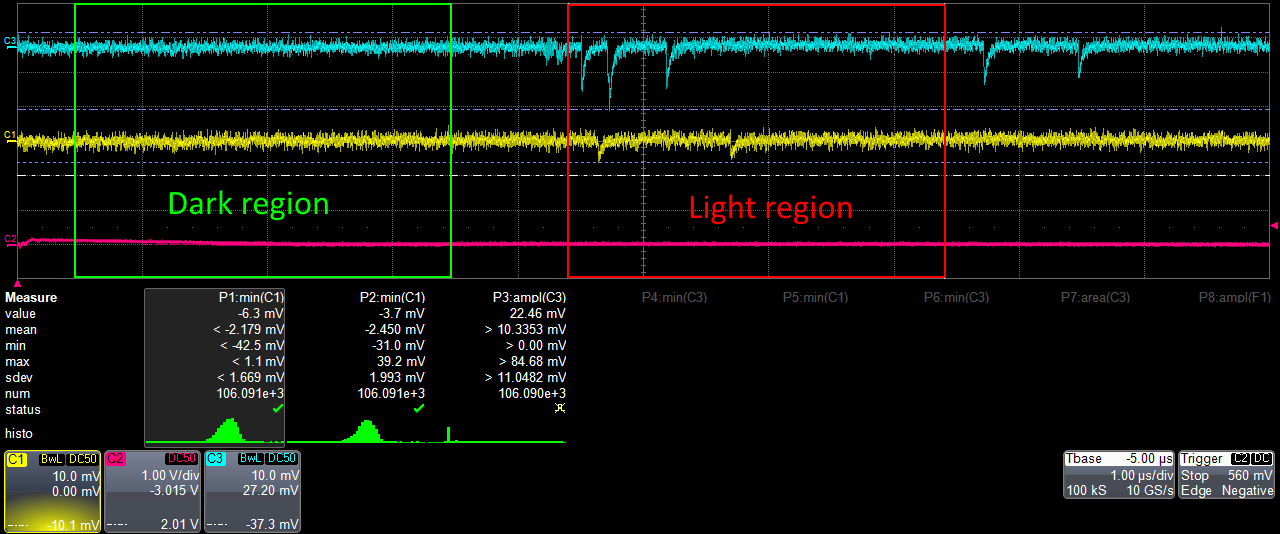
\includegraphics[totalheight=0.22\textwidth,trim=0cm 6.5cm 0cm 0cm, clip=true]{Pictures/blabla/light_region_3.png}
  \centering{\caption{Dark and light regions.}}
  \label{fig:dark_light_region}
  \end{figure}
  
  This error bar are quiet small (appendix for caculation). 
  
  \subsection{analyse : pont entre méthodoligie et solution }
  
  We would like to count the number of time we see a pulse corresponding to one PE peak. One PE peak match with detection of a photon firing 
  severals pixel and triggering an avalanches or show  DN. So in the light region it is not possible to make he difference between a pulse 
  from the detection of a photon or from DN. One way to take in account the pulse of DN is to use the dark region of the scope/waveform. 
  In that region we know for shure that one PE pulse comes obviously from DN.\\
  Considering the fact that DN in the light region or in the dark region appears at the same rate \footnte{follow poisson distribution,
  see appendix}, a solution will be to integrate the zero pe peak of the light and dark region. That's why our formula.
  
  It is obviously  clear that our results for  the PE stuff are not reproductible at all and this for lots reasons.
  
  \subsection{Influence of factors on PE stuff, issues}
  
  Three parameters could influence our results in the ``same'' experimental tets.
  
  \paragraph{the light}
  
  The volatge applied on the falsh lamp increase or decrease the light reaching the detectors. Also the position of the light (far or close of 
  the detector) has an influence. Speak about photon in N2? 
  The voltage of the lamp and the position on the lamp was set. 
  
  \paragraphe{the alignemeent} 
  
  The alignement of the detector with the lamp has an influence on the PE. We noticed the detector of the top wasn't properly aligned with the 
  one of the bottom. 
  
  picture with hole of 1mm. 
  
  \paragraph{the quantity of N2}
  
  The photon can propagate on a distance of mm  in oxygen but on a distance of in N2. That's why we used N2. 
  
  \paragraph{the tempearature}
  
  Th efficiency depend on temperature since Dn depend on temperature \footnote{see section}. 
  The tempearture seem to have an effect on Bs. All the box is cooling. the consequence is that the detector of the top is moving. 
  
  At room temperature, the PE of the Top detector is not constant. the tempearture of the lamp change of 2 degree when the lamp is working. 
  Even is after stabilisation.
  
  
  
  \subsection{further solutions}
  alignement of the lamp. all the box in plastic. Isolate the lamp to avoid radio leak. N2 near the detector. 
  effect of the dust on detecor right bu effect iwth light ? 
  
  
  \chapter{synthèse de l'avancement du proet}


  \chapter{Professional evaluation/Professionla statement}
  
  This internship was really benefit for me. I asked my co-workers 
  lots of questions because they had already worked on that project in the past. 
  I put my theoritical knowledges of matter physics and of detectors physics in pratics during 
  this internship. 
  \\
  
  I have also delighted to my skills learned in differents courses : 
  electronics, analysize and synthesis, research. This internship was 
  a real opportunity to increase my work, with more rigourus and with more method. 
  \\
  
  I was als happier to see that our work had a real impact on. I could saw that/ 
  I was able to see that my work was important for the advancement of the global project. 
  
  \chapter{Human evaluation/Human statement}
  
  From the beginning of my internship I tried to do my best to finish our project on time. 
  The goal was to publish something about my (our) work. This was a real motivation. 
  \\
  
  Also fro the beginning I real enjoyed working with my team. I can confirm that
  discussion moin formel. 
  \\
  
  Finally I really enjoyed my stay in Canada and espcially hiking, speaking english
 discover another culure at work or at home. 
 
 \chapter{conclusion 1 et recommandations}
  
  \\
  
  
 

%%%%%%%%%%%%%%%%%%%%%%%%%%%%%%%%%%%%%%%%%%%%%%%%%%%%%%%%%%%%
%                   bibliography                           %
%%%%%%%%%%%%%%%%%%%%%%%%%%%%%%%%%%%%%%%%%%%%%%%%%%%%%%%%%%%%
\begin{thebibliography}{999}
  \bibitem{ref:modern_particle_physics} Mark Thomson, \textit{Modern Particle Physics}, Hardcover,Oct 21 2013.
 \bibitem{ref:Fondamental_satistical_and_thermal_physics} Double beta decay, \url{http://www2.warwick.ac.uk/study/csde/gsp/eportfolio/directory/crs/phsgbu/research/phdresearch/theory/betadecay/double/}.
 \bibitem{ref:SiPM} Characterisation studies of silicon photomultipliers, {\em LATEX}, 2010, available at \url{http://arxiv.org/abs/1003.6071}.
 \bibitem{ref:DN} Dark Current in Silicon Photomultiplier Pixels: Data and Model, {\em LATEX}, 2012, available at \url{http://www.researchgate.net/publication/258656356_Dark_Current_in_Silicon_Photomultiplier_Pixels_Data_and_Model}.
 \bibitem{ref:CT} Modeling crosstalk in silicon photomultipliers, {\em LATEX}, 2013, available at \url{http://arxiv.org/abs/1302.1455}.
 \bibitem{ref:nEXO} Characterization of Silicon Photomultipliers for nEXO, {\em LATEX}, 2013, available at \url{http://arxiv.org/abs/1502.07837}. 
\end{thebibliography}


%%%%%%%%%%%%%%%%%%%%%%%%%%%%%%%%%%%%%%%%%%%%%%%%%%%%%%%%%%%%
%                    appendix                              %
%%%%%%%%%%%%%%%%%%%%%%%%%%%%%%%%%%%%%%%%%%%%%%%%%%%%%%%%%%%%
\appendix

%%%%%%%%%%%%%%%%%%%%%%%%%%%%%%%%%%%%%%%%%%%%%%%%%%%%%%%%%%%%
%                    appendix : nEXO                       %
%%%%%%%%%%%%%%%%%%%%%%%%%%%%%%%%%%%%%%%%%%%%%%%%%%%%%%%%%%%%

\chapter{The nEXO experiement}\label{app:nEXO}
  
  
  \section{the neutrinoless double beta decay : \(0\Pneutrino\beta\beta\)}
  
  \paragraph{\underline{\emph{History.}}}
  
  If this reference \cite{ref:wikipedia_beta} could give more details about the \(0\Pneutrino\beta\beta\), the double beta decay, which can proceed without 
  emission of any neutrino, was discovered by W. H. Furry in 1939. 

  \paragraph{\underline{\emph{Majorana particle and leptonic number violation.}}}
  
  To explain the \(0\Pneutrino\beta\beta\), lets start by reminding the double \(2\Pneutrino\beta\beta\) according the Standard Model. 
  As two neutrons become in two protons, the conservation of the charge implies the creation of two electrons \ref{eq:charge}. As 2 electrons appear, 
  the conservation of the leptonic electronic number implies the creation of two anti-neutrino \ref{eq:leptonic}:  
  
  \begin{equation} \label{eq:charge}
    (A,Z) \rightarrow (A,Z+2) + 2\Pelectron + 2\APneutrino
  \end{equation}
  leptonic electronic conservation :
  \begin{equation} \label{eq:leptonic}
    0 \rightarrow 0 + 2*(+1) + 2*(-1)
  \end{equation}
  
  Now lets consider the case when neutrinos are Majorana particles \footnote{ In opposition of Dirac particles where particles are distinct from anti-particles.}
  which means particles and anti-particles are identical except for their helicities. If so switching the helicity in this way allows 
  a particle in one frame of reference to be an anti-particle in another.
  \\
  That means that the emitted anti-neutrinos is neutrinos which conducts to the equation :
  
  \begin{equation}
    (A,Z) \rightarrow (A,Z+2) + 2\Pelectron + 2\Pneutrino
  \end{equation}
  
  Here we can observe the lepton number violation which would be an observation of ``Physics beyond the standard model'' :
  
  \begin{equation}
    0 \rightarrow 0 + 2*(+1) + 2*(+1)
  \end{equation}
  
  The Feyman diagrams related to \(2\Pneutrino\beta\beta\) and \(0\Pneutrino\beta\beta\) would be \cite{ref:beta_decay}: 
  
  \begin{figure}[!hbtp]
  \centering
  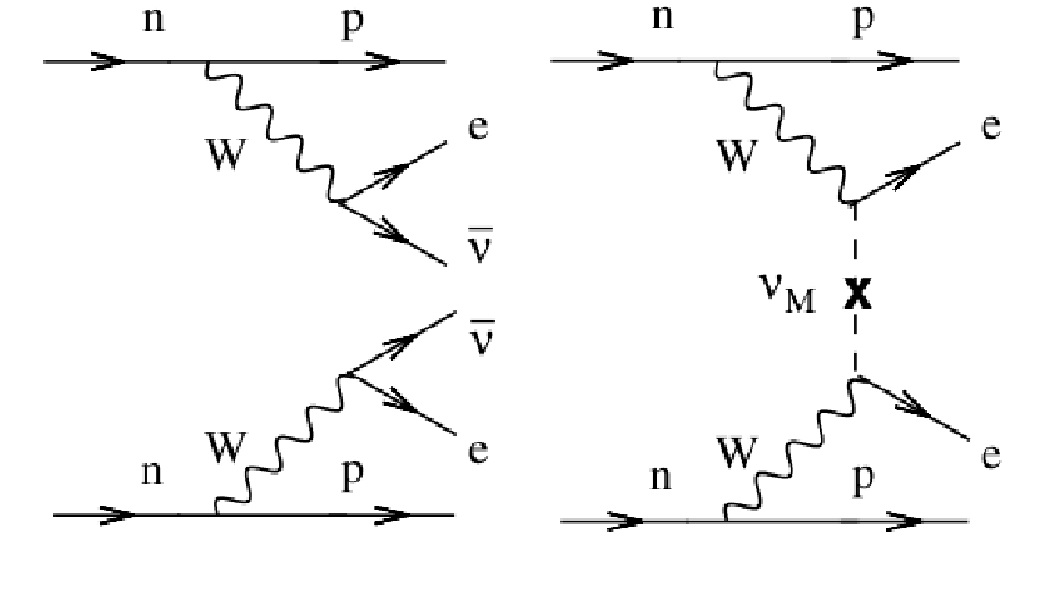
\includegraphics[totalheight=0.5\textwidth,trim=0cm 0cm 0cm 0cm, clip=true]{Pictures/blabla/beta.jpg}
  \centering{\caption{The \(2\Pneutrino\beta\beta\) (left) and the \(0\Pneutrino\beta\beta\) (right) : a virtual \Pneutrino instead of two \APneutrino.}
  \label{fig:feyman}
  \end{figure}
  
  \paragraph{\underline{\emph{The  measurement of the neutrino mass}}}
  If neutrinoless double beta decay were observed, it would also provide a measurement of the neutrino mass, since the rate of neutrinoless double beta 
  decay is related to the square of the neutrino mass : 
  
  \begin{equation}
    \Gamma = ~~~~{G |M|^2 |m_{\beta \beta}|^2}, with m_{\beta \beta} = \sum_{i=1}^3 m_i U^2_{ei}. 
  \end{equation}
   
  where G is the two-body phase-space factor, M is the nuclear matrix element and mββ is the effective Majorana neutrino.


  \section{The nEXO experiment}

  The \(2\Pneutrino\beta\beta\) or the  \(0\Pneutrino\beta\beta\) releases two electrons with a high energy (kinetic energy).   
  The \ce{^{136}Xe} is then in an existed state. It relaxes by releasing a photon. 
 
  Then the relased photon enters inside a SiPM. The photoelectric effect happens and the avalanche process begins. 
  \\
  
  The nEXO experiment consist in a big barrel whose walls are covered by SiPMs. This barrel will be filled with 5 tonnes of Xe liquid : 
  
  \begin{figure}[!hbtp]
  \centering
  \includegraphics[totalheight=0.5\textwidth,trim=0cm 0cm 10cm 0cm, clip=true]{Pictures/nEXO_barrel.png}
  \centering{\caption{The nEXO barrel.}}
  \label{fig:nEXO_barrel}
  \end{figure}
  

  
  Founded in 1968 and located on the campus of the University of British Columbia,\TR is one of the world’s leading subatomic physics laboratories 
  and the first national laboratory in Canada. The main feature of this laboratory is a cyclotron which was built in 1971. 
  While maintaining ties to the research programs among the 19 different member unversities from across Canada, this large community, composed of 
  international teams of scientists, post-doctoral fellow and students, has expanded from nuclear physics 
  to particle physics, molecular and materials science, and nuclear medicine.
  \\
  
  Among the particle physcics collaboration hosted by \TR is nEXO, whose goal is to search for evidence of the theoritical 
  neutrino-less double beta decay \(0\Pneutrino\beta\beta\). The standard model predicts the ordinary double beta decay \(2\Pneutrino\beta\beta\). The 
  detection of \(0\Pneutrino\beta\beta\) would validate ``Physics beyond the standard model'', show that the neutrino is a Majorana particle and 
  give a measure of the absolute neutrino mass. 
  \\
  
  \ce{^{136}Xe} is one of the 35 natural isotopes capable of \(2\Pneutrino\beta\beta\). If \(0\Pneutrino\beta\beta\) is possibleot would occur in \ce{^{136}Xe} 
  according to this reaction : 
    
  %\begin{equation}
    \ce{^{136}Xe} \rightarrow \ce{^{136}Ba} + 2\Pelectron %\iff 2\Pneutron \rightarrow 2\Pproton + 2\Pelectron \iff \ce{^{136}Xe} \rightarrow 2\APneutrino + 2\Pelectron 
  %\end{equation}
   
  The two electrons, which are ejected with high kinetic energy, scatter off the electrons of other \ce{^{136}Xe} atoms. If so, one of the impacted \ce{^{136}Xe}
  atoms is excited from the ground state and then de-energizes by releasing photons. This is knowen as scintillation. The wavelength of the created light is 175 nm. 
  \\
  
  So nEXO is currently being designed to use 5 tons of enriched liquid Xenon contained in a barrel. The wall of this barrel is covered with SiPM detectors. 
  \footnote{Silicum Photo-Multiplier.}
  \\  
  The goal of my research internship is to indentify suitable SiPMs for nEXO by testing devices from several manufacturers. In 2014 a test setup 
  was built: a box divided in two parts. The first part contains a \xfl which sends photons to the surface of two SiPM detectors. The signals are observed 
  on the screen of an oscilloscope, which is monitored by a computer to register and store waveforms. An algorithm (C++ and root) lets us characterize the SiPMs.
  \\
  
  So the question is to know if the selected SiPM could fufill all the experiment's requirements: achieve efficiency \(\geq\)15\% at 175nm (the wavelength 
  of Xenon scintillation), achieve dark noise rate less than 50Hz/mm\texttwosuperior{} and limit the number of correlated pulses (cross-talk and after-pulse)  
  to less than 0.02 per parent pulse.
  
  If the first part will describe briefly the nEXO experiment and remind the reader how  a SiPM works, the second part will give more details about the setup 
  and the algorithm. This would allow the results in the third part to be understood. 
  
 
  will saturatebeing tested is critical to receiving good data. The measurements
  being taken rely on observing a maximum of one photon over a given time
  interval that is determined by the response of individual detectors. For instance, a
  particular silicon photomultiplier (SiPM) may respond to a single photon with a
  pulse that spans 700 ns. In this scenario, the SiPM must not receive more light
  than the case where one photon every 700 ns is observed, otherwise saturation of
  the signal occurs and good data cannot be acquired. Figure 1 illustrates an
  acceptable signal, and a saturated signal, for one of the SiPMs to be tested. As a
  2result of this light output requirement, the Xenon flash lamp must be
  commissioned to only allow a limited amount of light into the system.

  The simplest method for controlling light output for the system is through
  movement. Intensity of light drops off as one over distance squared, and thus
  motion of the lamp will affect the number of photons hitting the detectors.
  Control over the flash lamp location is provided by a rod attached to the lamp
  mount and extending out of the box through a port. In the test set-up, this allows
  for approximately a 20 cm range of movement to and from the photodetector
  candidates. A simple comparison between lamp positions found that this motion
  can change the light output by a factor of four.

  he effect of using filters in the set-up was tested with filters from eSource
  Optics, Pelham Research Optical, and THORlabs by comparing the charge build-
  up on a reference multipixel photon counter (MPPC) and a photo multiplier tube
  (PMT) with the flash lamp light being both filtered and unfiltered. 4,5,6 The results
  are presented below in Table 1. Overall, no significant difference was found
  between the UV filters' transmission; the UV filters from Pelham and the UV
  filter from eSource all resulted in similar charge-build up, reducing the charge
  received by the MPPC and PMT by a factor of 10 000. As a contrast, the visible-
  4range filter reduced the charge by a factor of 100. This is an expected result, due
  to the spectrum of the lamp peaking around 400 nm.

  The L9455 and L9456 are compact xenon flash lamp modules integrating a 5-watt xenon flash lamp with its power supply and trigger socket.
  These lamp modules allow an energy input up to 5 watts, which is the maximum among similar lamp modules of the same size

%%%%%%%%%%%%%%%%%%%%%%%%%%%%%%%%%%%%%%%%%%%%%%%%%%%%%%%%%%%%
%                    appendix : SiPM                       %
%%%%%%%%%%%%%%%%%%%%%%%%%%%%%%%%%%%%%%%%%%%%%%%%%%%%%%%%%%%%

%\chapter{Few details about SiPM}\label{app:SiPM}

  APDs (Avalanche Photodiodes) are high-speed, high sensitivity photodiodes utilizing an internal gain mechanisme that function as reverse voltage. 
  
  Passive quenching : The avalanche photodiode (i.e. each pixel for the silicon photomultiplier) is
connected to the power supply through a large series resistor R s ( R s ≈ 100 − 400kΩ accord-
ing the manufacturer). If the current through the diode equals zero, the voltage across the diode
equals U bias , which is larger than the breakdown voltage. If the diode breaks down, the series
resistor reduces the voltage across the APD, what quenches the avalanche. After the breakdown is
quenched, the diode is recharged through the resistor. A drawback of passive quenching is then the
slow recharge of APD.

%\paragraph{more detail about dark noise}

%\paragraph{Principe of APD}

%\paragraph{part about anti-reflective glass and csq}


  
  
  During an avalanche, only a very small fraction of the trapping level is filled : therefore, the trap population is always well below saturation and 
  the carrier trapping probability remains constant during all the avalanche pulse. 
  
  Each electron-hole recombination mechanism can be reverse leading to a carrier generation. Recombination holds when excess carriers decay. 
  Generation takes place when there is a paucity of carriers. We can distinguish three ways of recombination. 
  
  ∗ Band-to-band recombination or radiative recombination : electron-hole pairs recombine directly from band to band with the energy carried away by photons.
  An electron falls from its state in the conduction band into the empty state in the valence band which is associated with the hole. Its counterpart is the 
  optical electron-hole pairs generation.
  
  ∗ Trap assisted recombination, also called Shockley Read Hall effect: electron-hole pairs recombine through deep-level impurities. An electron falls 
  into a "trap", an energy level within the bandgap caused by the presence of a foreign atom or a structural defect. The electron occupying the trap can in 
  a second step fall into an empty state in the valence band, thereby completing the recombination process. One can envision this process either as a 
  two-step transition of an electron from the conduction band to the valence band or also as the annihilation of the electron and the hole which meet each other in the trap.
  The energy liberated during the recombination event is dissipated by lattice vibrations or
  phonons. Its counterpart is thermal electron-hole pairs generation
  
  ∗ Auger recombination: an electron and a hole recombine in a band-to-band transition,
  but the resulting energy is absorbed by a third carrier (another electron or hole). Its
  counterpart is the impact ionization.
  
  Usually, a recombination event needs a third partner to allow conservation of energy and crys-
  tal momentum. This third partner is often a lattice defect, most commonly an impurity atom,
  with an energy state deep in the band gap, i.e. not close to the band edge. Recombination is
  then determined by these deep states or deep levels (cf. [18]).


On this dark noise, some cross-talk is observed :
photons emitted by the pixel "fired" may migrate to other pixels and trigger avalanches (cf. §4.1
and §4.3.4). We calibrate on this dark noise.

picture histogram


  
  The probability that an afterpulse occurs increases with the amount of charge that flows through the diode during a Geiger
  discharge. Thus, the afterpulsing probability increases with increasing bias voltage.
 %introduction sentence for SiPM : 
  
 
  accurate  description  of  this effects :
  
    When a pixel is red by either an incoming photon or by a thermally generated electron-
  hole pair, hot carriers in the avalanche breakdown induce emission of IR photons [2{4] thatSiPM
  in turn may trigger further avalanches in nearby pixels.  This stochastic process,  called
  optical  cross-talk,  is  characterized  by  being  nearly  instantaneous,  and  its  probability  is
  proportional to the SiPM gain. Operating at low bias voltage would diminish signicatively
  cross-talk  eects,  but  at  the  expense  of  degrading  the  photon-detection  eciency.   The
  incorporation  of  isolation  trenches  around  each  pixel,  as  proposed  by  [5],  successfully
  reduces optical cross-talk [6{8].  This technique has become very usual in the fabrication
  of this kind of photodetectors.  However, it was rst shown in [9] that a very signicant
  contribution to cross-talk can come from light re
  ected on the bottom surface of the Si
  bulk, and thus, trenches would not be able to completely prevent it.
  The  main  eect  of  cross-talk  is  to  introduce  a  multiplication  noise,  although  it  does
  not aect the pulse-height resolution.  So, at conditions where only one pixel is expected
  to be excited simultaneously (e.g.,  dark counts),  cross-talk results in output pulses with
  amplitudes twice or several times the amplitude of a single triggered pixel.  The cross-talk
  probability
  "
  is usually dened as the rate of dark counts with cross-talk (two or more red
  pixels) divided by the total dark-count rate

  assuming that cross-talk only takes place between adjacent pixels

  including light propa-
  gation through the silicon bulk and re
  ections on the bottom surface, have demonstrated
  that cross-talk can also be induced in distant pixels, which is supported by experimental
  data for these SiPMs

  An analytical formulation is desirable for a better understanding of cross-talk eects

% \paragraph{After-Pulses}
  
  another issue: carriers trapped during the avalanche discharge and then released trigger a new avalanche during a period of several 100 ns after 
  the breakdown. After pulse increase with the biais volatage. 

  This array could resume why we have choosen Hammatsu \footnote{Appendix 2 gives a large comparaison between differents constructors.}
  
%\paragraph{other point of view  on three issues}

  dark noise : 
  \\
  The main source of noise limiting the SiPM performances is the dark noise rate, which mainly originates from the carriers created thermally in the 
  depletion layer.
  
  Each electron-hole recombination mechanism can be reverse leading to a carrier generation. Recombination holds when excess carriers decay. 
  Generation takes place when there is a paucity of carriers. We can distinguish three ways of recombination. 
  
  ∗ Band-to-band recombination or radiative recombination : electron-hole pairs recombine directly from band to band with the energy carried away by photons.
  An electron falls from its state in the conduction band into the empty state in the valence band which is associated with the hole. Its counterpart is the 
  optical electron-hole pairs generation.
  
  ∗ Trap assisted recombination, also called Shockley Read Hall effect: electron-hole pairs recombine through deep-level impurities. An electron falls 
  into a "trap", an energy level within the bandgap caused by the presence of a foreign atom or a structural defect. The electron occupying the trap can in 
  a second step fall into an empty state in the valence band, thereby completing the recombination process. One can envision this process either as a 
  two-step transition of an electron from the conduction band to the valence band or also as the annihilation of the electron and the hole which meet each other in the trap.
  The energy liberated during the recombination event is dissipated by lattice vibrations or
  phonons. Its counterpart is thermal electron-hole pairs generation
  
  ∗ Auger recombination: an electron and a hole recombine in a band-to-band transition,
  but the resulting energy is absorbed by a third carrier (another electron or hole). Its
  counterpart is the impact ionization.
  
  Usually, a recombination event needs a third partner to allow conservation of energy and crys-
  tal momentum. This third partner is often a lattice defect, most commonly an impurity atom,
  with an energy state deep in the band gap, i.e. not close to the band edge. Recombination is
  then determined by these deep states or deep levels (cf. [18]).
  
  about after-pulse : Trapping phenomena - Afterpulsing

  Traps may result from the damage caused by an implantation in the fabrication process.
  Deep levels trap some avalanche carriers and release them with a statistical delay. If the
  delay is greater than the dead time after the previous avalanche pulse, a released carrier can
  re-trigger an avalanche and cause a statistically correlated pulse. 
  These carriers, captured by trapping centers inside the depletion layer and released after the diode has been recharged,
  form the afterpulse. 
  
  During an avalanche, only a very small fraction of the trapping level is filled : therefore, the trap population is always well below saturation and 
  the carrier trapping probability remains constant during all the avalanche pulse. 
  
  The probability that an afterpulse occurs increases with the amount of charge that flows through the diode during a Geiger
  discharge. Thus, the afterpulsing probability increases with increasing bias voltage.
  
   
  
  

  
  %create an appendix for that ? 
  %Here we can observe the lepton number violation which would be an observation of ``Physics beyond the standard model'' :
  
  %\begin{equation}
    %0 \rightarrow 0 + 2*(+1) + 2*(+1)
  %\end{equation}
  
  %The Feyman diagrams related to \(2\Pneutrino\beta\beta\) and \(0\Pneutrino\beta\beta\) would be \cite{ref:beta_decay}: 
  
  %\begin{figure}[!hbtp]
  %\centering
  %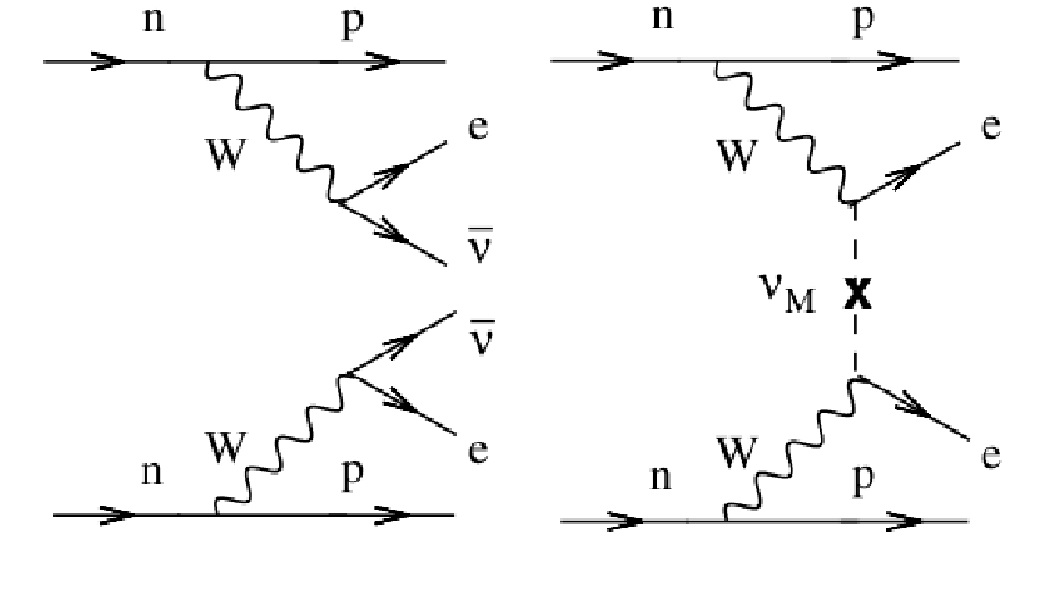
\includegraphics[totalheight=0.5\textwidth,trim=0cm 0cm 0cm 0cm, clip=true]{Pictures/blabla/beta.jpg}
  %\centering{\caption{The \(2\Pneutrino\beta\beta\) (left) and the \(0\Pneutrino\beta\beta\) (right) : a virtual \Pneutrino instead of two \APneutrino.}
  %\label{fig:feyman}
  %\end{figure}
  
  
  
  If neutrino is a Majorana particle, that means 
 Possible  if the decay endpoint large enough which means Q>2 Mev). 
 
  If \(0\Pneutrino\beta\beta\) is possible, 
  it would occur in \ce{^{136}Xe} according to this reaction : 
    
  \begin{equation}
    \ce{^{136}Xe} \rightarrow \ce{^{136}Ba} + 2\Pelectron %\iff 2\Pneutron \rightarrow 2\Pproton + 2\Pelectron \iff \ce{^{136}Xe} \rightarrow 2\APneutrino + 2\Pelectron 
  \end{equation}
   
  The two electrons, which are ejected with high kinetic energy, scatter off the electrons of other \ce{^{136}Xe} atoms. If so, one 
  of the impacted \ce{^{136}Xe} atoms is excited from the ground state and then de-energizes by releasing photons. 
  This is knowen as scintillation process. The wavelength of the created light is 175 nm. 
  \\
  %% presentation thesis
  
  Current limits on the half-life of \(0\Pneutrino\beta\beta\) are > 10up(25) yr, providing a 
  formidable challenge. The Enriched Xenon Observatory (EXO) is a 
  double beta decay experiment poised to improve upon this limits, using
  xe136 as both a source and detector of this decay. \(0\Pneutrino\beta\beta\) of xe136 produces a detectable
  energy deposition....
  
  One possible method of measuring the neutrino mass is by observation of a rare, 
  as yet unseen, second order electroweak process called neutrinoless double 
  beta decay (\(0\Pneutrino\beta\beta\)). \\
  EXO is designed to search for thsi decay in xe136. In the standard version
  of this process (\(2\Pneutrino\beta\beta\)) a xe 136 decays to a ba136++, emitting two electrons and two anti-neutrinos. 
  This process has been observed in various nuclei, but doesnot allowfor a measuremetn
   of absolute neutrino mass. 
   
  
 beta decay is the simplest method of making an absolute neutrino mass measurement. 
 \(0\Pneutrino\beta\beta\) has the potential to probe mass limits in the meV range (combining cosmological and oscillation
 results, one neutrino mass should be in the range mvelec = (0.04-0.1) ev. Confirmation by 
 exo in ...), provided neutrinos are Majorana particles, ad lepton number
 conservation is violated. 
 \(0\Pneutrino\beta\beta\) is  due to the exchange of light Majorana neutrinos, the neutrino mass
 spectrum is strongly degenerate . 
 
 % double beta decay thesis
 
 Two neutrino double beta decay (\(2\Pneutrino\beta\beta\)) is a standard second-order electroweak
 process, whereby a nucleus with charge Z and mass number A decays to a nucleus
 with charge Z+2 and mass numberA, where both Z and A are even. We speak about even-even nuclei (like evn-odd nuclei or odd-odd nuclei). 
 
 \begin{equation} \label{eq:charge}
    (A,Z) \rightarrow (A,Z+2) + \Pelectron1 + \Pelectron2 + \APneutrino1 + \APneutrino2
 \end{equation}
 
 Z is the number of proton and A is the number of proton and neutron. As ``rien ne se pert, rien ne se cre, tout se transforme'', 
 the equation above means that in this process, 2 neutrons decay to 2 protons. 
 
 The array of section above and the conservation of the charge \footnote{rule in physics} 
 implies the creation of two electrons \ref{eq:charge}. \\
 
 As 2 electrons appear and according to the array above, the conservation of the leptonic electronic number \footnote{another rule} 
 implies the creation of two anti-neutrino \ref{eq:leptonic}:  
 \begin{equation} \label{eq:leptonic}
    0 \rightarrow 0 + 2*(+1) + 2*(-1)
 \end{equation}
  
 So the equation is right. 
 
 Now the total energy difference (which is difference between mass. Mass of particle are expressed in energy since einstein low
 direct relation/tie between mass and energy) between the initial and final nuclei
 is called the Q-value. In \(2\Pneutrino\beta\beta\), this energy is distributed among the emitted electrons, neutrinos, and nuclear 
 recoil of the daughter nucleus. As it has been said, this process occurs in various
 'even-even`` nuclei, with a certain rate. This rate would be dwarfed by the single 
 beta-decay rate, if it were not for a perculiarity in the nuclear mas function of certain
 even-even nuclei. This is shown for the case of xe136 in fig. number where single beta-decay to cs136 is energetically disfavored
 over \(2\Pneutrino\beta\beta\) to ba 136++. Possible  if the decay endpoint large enough which means Q>2 Mev). 
 
 This process is observed experimentally via the sum electron energy spectrum. 
 The electron energy spectrum of \(2\Pneutrino\beta\beta\) is continous, as the neutrino can be emitted with a kinetic
 energy between 0 and Q. 
 
 Complete it. 
 
 2 isotopes provides in particular a means of eliminating radioactive back-grounds. 
 \(0\Pneutrino\beta\beta\) of xe 136 produces 136 ba++(which become 136 ba+ by capturing an electron from the lXe conduction
 band) which can be identified via resonance fluorescence immadiately after the decay. The 
 EXO-200 and EXO experiements, described below, look for  \(0\Pneutrino\beta\beta\) using xe136. 
  
  %% other presentation
  To explain the \(0\Pneutrino\beta\beta\), lets start by reminding the double \(2\Pneutrino\beta\beta\) according the Standard Model. 
  As two neutrons become in two protons, the conservation of the charge implies the creation of two electrons \ref{eq:charge}. As 2 electrons appear, 
  the conservation of the leptonic electronic number implies the creation of two anti-neutrino \ref{eq:leptonic}:  
  
  \begin{equation} \label{eq:charge}
    (A,Z) \rightarrow (A,Z+2) + 2\Pelectron + 2\APneutrino
  \end{equation}
  leptonic electronic conservation :
  \begin{equation} \label{eq:leptonic}
    0 \rightarrow 0 + 2*(+1) + 2*(-1)
  \end{equation}
  
  Now lets consider the case when neutrinos are Majorana particles \footnote{ In opposition of Dirac particles where particles are distinct from anti-particles.}
  which means particles and anti-particles are identical except for their helicities. If so switching the helicity in this way allows 
  a particle in one frame of reference to be an anti-particle in another.
  \\
  That means that the emitted anti-neutrinos is neutrinos which conducts to the equation :
  
  \begin{equation}
    (A,Z) \rightarrow (A,Z+2) + 2\Pelectron + 2\Pneutrino
  \end{equation}
  
  Here we can observe the lepton number violation which would be an observation of ``Physics beyond the standard model'' :
  
  \begin{equation}
    0 \rightarrow 0 + 2*(+1) + 2*(+1)
  \end{equation}
  
  The Feyman diagrams related to \(2\Pneutrino\beta\beta\) and \(0\Pneutrino\beta\beta\) would be \cite{ref:beta_decay}: 
  
  \begin{figure}[!hbtp]
  \centering
  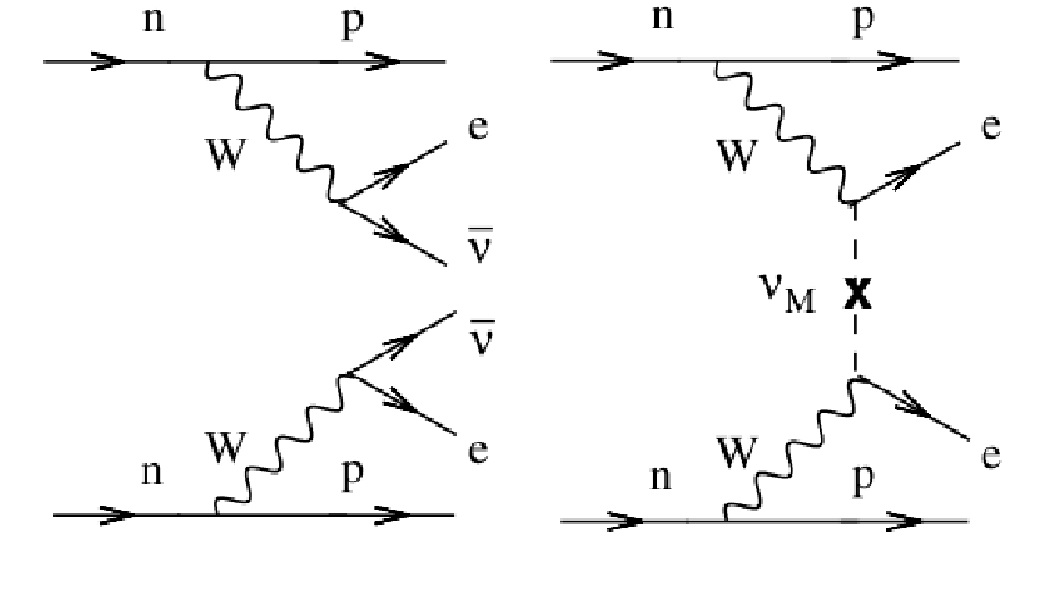
\includegraphics[totalheight=0.5\textwidth,trim=0cm 0cm 0cm 0cm, clip=true]{Pictures/blabla/beta.jpg}
  %\centering{\caption{The \(2\Pneutrino\beta\beta\) (left) and the \(0\Pneutrino\beta\beta\) (right) : a virtual \Pneutrino instead of two \APneutrino.}
  \label{fig:feyman}
  \end{figure}
  
  
  Recent neutrino oscillation results provide experimental proof that neutrinos 
  are massive particles. These measurement, however, reveal information about 
  neutrino 
  
  
EXO's experiment is looking for neutrinoless double beta decay in the 136 isotope of xenon. The experiment currently consists of 
  two facets:

    EXO-200, a 200-kilogram prototype experiment currently operating at WIPP. It has measured for the first time the two-neutrino mode 
    of double beta decay of Xenon 136. It has also set the most stringent limit on the rate of neutrinoless double beta decay. 
    It continues to collect data in order to improve on this limit or potentially discover the decay.
    nEXO, ("next EXO"), a tonne scale experiment using Xenon 136 to search for neutrinoless double beta decay. The collaboration is 
    undergoing extensive R&D to design the xenon detector and a way to "tag" the barium daughter ion produced by the decay in order 
    to eliminate all backgrounds.

  There are many advantages to using a noble element, specifically xenon. It is relatively easy to purify the LXe, which allows it to 
  be reused in different detectors. The 136 isotope can be enriched using the same centrifuge techniques used for fissile nuclear isotopes,
  which makes processing large quantities feasible, while putting the centrifuges to peaceful use. The xenon 136 Q-value — the energy of 
  the decay — is 2.48 MeV, which is high enough to be above many of the uranium gamma lines. Gamma rays from naturally-occurring 
  radioactive isotopes are a background that can make the decay we're interested in difficult or impossible to detect. Nobel liquids 
  like LXe are natural radiation detectors, and so we avoid the need for excess materials that could generate extra radioactive 
  backgrounds. Furthermore, we are able to achieve great energy resolution through collecting both ionization electrons and scintillation
  light from the xenon. Finally, xenon potentially allows for complete background rejection through tagging of the daughter Barium ion. 
  This unique property motivates much of the work done by our collaboration.
  \\
 
%%%%%%%%%%%%%%%%%%%%%%%%%%%%%%%%%%%%%%%%%%%%%%%%%%%%%%%%%%%%
%%%%%%%%%%%%%%%%%%%%%%%%%%%%%%%%%%%%%%%%%%%%%%%%%%%%%%%%%%%%
%%%%%%%%%%%%%%%%%%%%%%%%%%%%%%%%%%%%%%%%%%%%%%%%%%%%%%%%%%%%
%%%%%%%%%%%%%%%%%%%%%%%%%%%%%%%%%%%%%%%%%%%%%%%%%%%%%%%%%%%%
... pr\'ec\`ede un nouveau chapitre.

%%%%%%%%%%%%%%%%%%%%%%%%%%%%%%%%%%%%%%%%%%%%%%%%%%%%%%%%%%%%
%%%%%%%%%%%%%%%%%%%%%%%%%%%%%%%%%%%%%%%%%%%%%%%%%%%%%%%%%%%%
%%%%%%%%%%%%%%%%%%%%%%%%%%%%%%%%%%%%%%%%%%%%%%%%%%%%%%%%%%%%
... pr\'ec\`ede une nouvelle section.

%%%%%%%%%%%%%%%%%%%%%%%%%%%%%%%%%%%%%%%%%%%%%%%%%%%%%%%%%%%%
%%%%%%%%%%%%%%%%%%%%%%%%%%%%%%%%%%%%%%%%%%%%%%%%%%%%%%%%%%%%
...pr\'ec\`ede une nouvelle sous-section.

%%%%%%%%%%%%%%%%%%%%%%%%%%%%%%%%%%%%%%%%%%%%%%%%%%%%%%%%%%%%
...pr\'ec\`ede une nouvelle sous sous-section.


remplacer avec Ctrl + R, une fois que le document est fini de r\'edig\'e.
caract\`eres :
'	'
à	\`a
â	\^a
é	\'e
è	\`e
ê	\^e
ù	\`u
ô	\^o
î	\^i
ï	\"i
ç	\c c
œ	\oe{}
²	\texttwosuperior{}
>	\textgreater
"	\og	(ouvrant)
"	\fg{}	(fermant)

 %{\qtreeshowframes
  \Tree 
    [.Head of \TR: \textit{\textcolor{blue}{Dr. Jonathan BAGGER} } 
      [.Head of Science Division: \textit{Dr. Reiner KRUECKEN} 
	[.Head of Science technology: \textit{Dr. Fabrice RETIERE} 
	  [.Head of Developement: \textit{Dr. Fabrice RETIERE} 
	  [.Developement of photo-detectors for nEXO: \textit{Dr. Fabrice RETIERE} {Carl RETHMEIER} {Llyod JAMES} {Paul LOPES GOMES} !{\qbalance}] %last !{\qbalance} 
	  ] 
	] 
      ]	
    ] 
  %}
  %}